% Authors: Simon Geoffroy-Gagnon and Farhad Shokraneh
% Based on the Thesis by Rubana Bahar Priti
% Edit: 2020.04.16

\documentclass[12pt, TexShade, letterpaper]{report}
\usepackage[utf8]{inputenc}
\usepackage{palatino}
\usepackage{amsmath}
\usepackage{amssymb} 
\usepackage{graphicx}
\usepackage[labelfont=bf]{caption}
\usepackage{subcaption}
\usepackage{setspace}
\captionsetup[table]{font = {stretch=1.35}}
\captionsetup[figure]{font = {stretch=1.35}}
\usepackage[margin=1in, headsep=1cm, bottom=5cm]{geometry}
%\usepackage[hidelinks]{hyperref}
%\usepackage[colorlinks=true]{hyperref}
\usepackage{hyperref}
%\newcommand{\MYhref}[3][blue]{\href{#2}{\color{#1}{#3}}}%
\usepackage{tabu}
%\usepackage{cite}
\usepackage[table]{xcolor}
%\usepackage{nomencl}
%\usepackage[nonumberlist,nogroupskip,xindy]{glossaries}
\usepackage{floatrow}
\usepackage{wrapfig}
\renewcommand{\baselinestretch}{2} 
\usepackage{fancyhdr}
\usepackage{lmodern}
\usepackage{titlesec}
\usepackage[natbib,style=numeric-comp,backend=biber,sorting=none]{biblatex}

\usepackage{times}

\definecolor{quotationcolour}{HTML}{F0F0F0}
\definecolor{quotationmarkcolour}{HTML}{1F3F81}

\addbibresource{phd_thesis.bib}

%%%%%%%%%%%%%%%%%%%
%
% FORMATTING HEADERS
%
%%%%%%%%%%%%%%%%%%%

% Format spacing around headers

%\titlespacing*{<command>}{<left>}{<before-sep>}{<after-sep>}
%\titleformat{<command>}[<shape>]{<format>}{<label>}{<sec>}{<before-code>}[<after-code>]

% Reduce gap between chapter header and chapter title
\titleformat{\chapter}
            [hang] %shape 
            {\vspace{-2cm}\bfseries\Large}
            {\thechapter}
            {20pt} % distance between number and title
            {} 
            []
            
% Make section titles a bit smaller than chapter titles
\titleformat{\section}
            [hang] %shape 
            {\bfseries\large}
            {\thesection}
            {20pt} % distance between number and title
            {} 
            []
            
\titleformat{\subsection}
            [hang] %shape 
            {\bfseries\normalsize}
            {\thesubsection}
            {20pt} % distance between number and title
            {} 
            []
            
\titlespacing*{\chapter}{0pt}{5.5ex plus 1ex minus .2ex}{0pt}

\titlespacing*{\section}
{0pt}{5.5ex plus 1ex minus .2ex}{0pt}

\titlespacing*{\subsection}
{0pt}{5.5ex plus 1ex minus .2ex}{0pt}

% Command to prevent \chapter from numbering chapters
% Otherwise you get stuff like "CHAPTER 3: Chapter one"
\makeatletter
\newcommand{\unchapter}[1]{%
  \begingroup
  \let\@makechapterhead\@gobble % make \@makechapterhead do nothing
  \chapter{#1}
  \endgroup
}
\makeatother

%\renewcommand{\chaptermark}[1]{\markboth{#1}{}} % Ensure List of Figs, ToC, and glossary are named in the header

% Custom headers for List of figures/tables (removes capitalization)
\renewcommand{\listfigurename}{List of figures}
\renewcommand{\listtablename}{List of tables}

% Overwrite the plain page style with a red line and page numbering
\fancypagestyle{plain}{%
	\fancyhf{} % clear all header and footer fields
	\fancyhead[R]{\textbf{\thepage}} % except the center
}

% Create the fancy page style header
\pagestyle{fancy}
\fancyhf{}
\lhead{\textbf{\nouppercase{\leftmark}}}
\chead{}
\rhead{\textbf{\thepage}}

\usepackage{xpatch}
\xpretocmd\headrule{\color{red}}{}{\PatchFailed}

%\author{\textcopyright Author, August, 2020}
%\date{}

\setcounter{chapter}{-1}

\begin{document}

% trying to get chapters to stop appearing as roman numerals in \ref
% jfc why is htis so hard
% \renewcommand{\thechapter}{\arabic{chapter}}

%%%%%%%%%%%%%%%%%%%
%
% TITLE PAGE
%
%%%%%%%%%%%%%%%%%%%

\begin{titlepage}
\begin{center}

%\vspace*{0.5cm}



% {\sf\bfseries\LARGE  Data Consistency in Scalable\\
% Multi-tier Architectures}


% {\rm\bfseries\LARGE  Data Consistency}
% \vspace{0.15cm}
% {\rm\bfseries\LARGE  in}
% \vspace{0.15cm}
% {\rm\bfseries\LARGE  Multi-tier and Cloud Applications}

{\sf\bfseries\LARGE  The entangled biobank: On the topology of high-dimensional human genetic data }

%\vspace{0.15cm}

%{\sf\bfseries\LARGE  goes here}

%\vspace{0.15cm}

%{\sf\bfseries\LARGE  and here}

%\vspace{1.8cm}

\vspace{1.5cm}

{\large Alexandr Diaz-Papkovich}

\vspace{1.5cm}

%\vspace{1cm}

%\vspace{1.4cm}

Quantitative Life Sciences, McGill University\\
Montr\'{e}al, Qu\'{e}bec, Canada\\
August 2023

\vspace{1.5cm}



% \date{\today}

%\vspace{1.4cm}

\begin{figure}[H]
\centering

\includegraphics[width=0.4\columnwidth]{mcgill_sig_red.jpg}
\end{figure}

\vspace{1.5cm}

\noindent
A thesis submitted to McGill University in partial\\
fulfillment of the requirements of the degree of\\
Doctor of Philosophy


\vspace{1.4cm}

{\small \copyright Alexandr Diaz-Papkovich, 2023}


\end{center}
\end{titlepage}







 % Start of table of contents
\tableofcontents\thispagestyle{plain}

% Set page numbering to roman
\cleardoublepage
\setcounter{page}{1}\renewcommand{\thepage}{\roman{page}}	

%%%%%%%%%%%%%%%%%%%
%
% ABSTRACT
%
%%%%%%%%%%%%%%%%%%%

\chapter*{Abstract}\markboth{Abstract}{}
	\label{chap:engAbstract}
	\addcontentsline{toc}{chapter}{Abstract}  
	Oh god!

%%%%%%%%%%%%%%%%%%%
%
% FRENCH ABSTRACT
%
%%%%%%%%%%%%%%%%%%%

\chapter*{Abrégé}\markboth{Abrégé}{}
	\label{chap:frAbstract}
		\addcontentsline{toc}{chapter}{Abrégé}  
		Avec les progrès de la génomique, les biobanques sont en plein essor. Contenant les données génétiques de millions d'individus, les biobanques sont de riches dépôts, utilisés régulièrement et stimulant la découverte scientifique. Le génome humain s'étend sur environ trois milliards de paires de bases, ce qui fait de l'étude des données génétiques à grande échelle une tâche dans un espace de grande dimension. L'échelle même du problème est un défi, tout comme la complexité de la diversité génétique humaine. Grâce à de nouvelles méthodes d'analyse topologique des données, nous sommes en mesure de réduire la dimensionnalité de ces ensembles massifs de données tout en préservant d'importantes quantités d'informations à l'aide d'une méthodologie traçable à l'échelle de la biobanque.

Dans le cadre de cette recherche, nous appliquons «~uniform manifold approximation and projection~» (UMAP), une forme de la réduction de la dimensionnalité non linéaire, et HDBSCAN, un algorithme de regroupement basé sur la densité des données, à plusieurs biobanques de données génétiques humaines. Nous utilisons UMAP et HDBSCAN pour étudier la structure de la population, le phénomène dans lequel la variation génétique n'est pas aléatoire et est corrélée à des facteurs tels que la géographie, l'histoire démographique, la migration et la structure sociale. Nous développons une méthodologie qui nous permet de visualiser les données génétiques, d'identifier la structure de la variation génétique allant d'une poignée à des centaines de milliers d'individus. Nous découvrons des relations subtiles entre la génétique, l'histoire, la géographie et la distribution des phénotypes.

%%%%%%%%%%%%%%%%%%%
%
% ACKNOWLEDGEMENTS
%
%%%%%%%%%%%%%%%%%%%

\chapter*{Acknowledgements}\markboth{Acknowledgements}{}
	\label{chap:acknowledgments}
			\addcontentsline{toc}{chapter}{Acknowledgements}  
	This thesis would not have been possible without my many communities, nor without the contributions of those who donated their data to further our understanding of genetics.

I would like to thank Simon Gravel for his guidance and mentorship and his balance of energetic curiosity with scientific scepticism, and the members of my supervisory committee, Nada Jabado and Ryan Hernandez. I would also like to thank Celia Greenwood, the director of QLS, and Alex DeGuise, the co-ordinator, for all of their hard work.

Thank you to my QLS cohort for grinding it out with me: Myriah Haggard, Matt D'Iorio, Jeffrey Hyacinthe, Yixiao Zheng, and Sara Zapata-Marin; to Selin Jessa, for sending me down the rabbit hole; to Noor Al-Sharif and Jake Vogel, for making Montreal feel like home; to my Thomson House Trivia crew: Matt, Barbara, Hector, Gerardo, JT, Val, and Rozzy, for being champions; to the Gravel lab, especially my desk-mate Chief Ben-Eghan who always made me laugh.

Thank you to my friends in my other homes. Those in Ottawa: Dylan, Leo, Julie, Ashley, Shane, Isaac, Amy, thanks for always wanting to see me when I was in town. To my friends in KW: Jake, Kayla, Warren, Kaitlin, Jon, Steph, Derek, Christina, Dave, Rebecca, Tyler, and Aine, thanks for entertaining my rants on Slack---may your broods grow belligerent and numerous.

Thank you to my loved ones: to Melissa, for exploring the forests and rivers with me; to my brother, Andrew, and my mother, Marina, for carrying me when I stumbled; and lastly to my father, Andr\'{e}s, who started this marathon with me so long ago---the finish line is finally in sight, and I can hear you cheering.

\pagebreak
\hspace{0pt}
\vfill

\begin{center}
%\begin{minipage}{.7\linewidth}
In memory of Andr\'{e}s Carlos D\'{i}az Bravo.
%\end{minipage}
\end{center}

\vfill
\hspace{0pt}
\pagebreak


%%%%%%%%%%%%%%%%%%%
%
% CONTRIBUTION TO KNOWLEDGE
%
%%%%%%%%%%%%%%%%%%%

\chapter*{Contribution to original knowledge}\markboth{Contribution to original knowledge}{}
	\label{chap:knowledge}
			\addcontentsline{toc}{chapter}{Contribution to original knowledge}  
	The works presented in this thesis establish novel methodologies for dimensionality reduction, clustering, and visualization in population genetics with possible extensions to genomics at large. We explore applications of UMAP, a nonlinear dimensionality-reduction method, and HDBSCAN($\hat{\epsilon}$), a density-based clustering algorithm. The two methods form the basis of our topological data analysis. The approach is tractable, easy-to-implement, and fits in the paradigm of exploratory-confirmatory analysis of biobank data, particularly for large and complex cohorts.

In \hyperref[chap:chapter1]{Chapter~1} we apply UMAP to population genetic data for the first time. We establish that it efficiently reveals fine-scale population structure in biobanks and use it in data visualization in 2- and 3-dimensions. These visualizations correlate with a number of phenotypic, geographic, and socio-demographic measures, and often appear as clusters. As UMAP became popular in the field, in \hyperref[chap:chapter2]{Chapter~2} we review its use in population genetics and provide insights on its optimal use and potential downstream applications.

Finally, in \hyperref[chap:chapter3]{Chapter~3} we address algorithmic clustering of UMAP results. We apply HDBSCAN($\hat{\epsilon}$) to UMAP data in $3$ to $5$ dimensions and use it to stratify biobank data. We discover clusters of structure in genetic data and leverage them to study demographic histories of populations in biobanks, polygenic score transferability, phenotype distributions, identify potentially influential alleles, and its use in quality control.

%%%%%%%%%%%%%%%%%%%
%
% CONTRIBUTIONS OF AUTHORS
%
%%%%%%%%%%%%%%%%%%%

\chapter*{Contributions of authors}\markboth{Contributions of authors}{}
	\label{chap:authors}
			\addcontentsline{toc}{chapter}{Contributions of authors}  
	\section*{Chapter 2}
\begin{itemize}
\item \textbf{Alex Diaz-Papkovich}: Conceptualization, data curation, formal analysis, investigation, methodology, software, visualization, writing -- original draft, writing -- review \& editing 
\item \textbf{Luke Anderson-Trocm\'{e}}: Visualization
\item \textbf{Chief Ben-Eghan}: Data curation
\item \textbf{Simon Gravel}: Supervision, writing -- review \& editing
\end{itemize}

Acknowledgements: Audrey Grant, Ryan Hernandez, Jose Sergio Hleap, Mark Lathrop, Dominic Nelson, Markus Munter, Stephen Sawcer, Melissa Spear, and Dara Torgerson for useful discussions about science, programming, and data access; David Poznik, Liz Babalola, and Adam Auton for discussing findings in the 1KGP; Selin Jessa for introducing us to UMAP

\section*{Chapter 3}

\begin{itemize}
\item \textbf{Alex Diaz-Papkovich}: Conceptualization, data curation, formal analysis, investigation, methodology, software, visualization, writing -- original draft, writing -- review \& editing
\item \textbf{Luke Anderson-Trocm\'{e}}: Visualization, data curation
\item \textbf{Simon Gravel}: Supervision, writing -- review \& editing
\end{itemize}

\section*{Chapter 4}
\begin{itemize}
\item \textbf{Alex Diaz-Papkovich}: Conceptualization, data curation, formal analysis, investigation, methodology, software, visualization, writing -- original draft, writing -- review \& editing
\item \textbf{Shadi Zabad}: Software, data curation
\item \textbf{Chief Ben-Eghan}: Data curation
\item \textbf{Luke Anderson-Trocm\'{e}}: Visualization, data curation
\item \textbf{Georgette Femerling}: Data curation
\item \textbf{Vikram Nathan}: Methods testing
\item \textbf{Jenisha Patel}: Methods testing
\item \textbf{Simon Gravel}: Supervision, writing -- review \& editing
\end{itemize}

Acknowledgements: Claude Bh\'{e}rer, Melissa Spear, and Paul Verdu for scientific discussion.

%%%%%%%%%%%%%%%%%%%
%
% LIST OF ACRONYMS
%
%%%%%%%%%%%%%%%%%%%

\chapter*{List of abbreviations}\markboth{List of abbreviations}{}
	\label{chap:abbrevs}
			\addcontentsline{toc}{chapter}{List of abbreviations}  
	%\addcontentsline{toc}{chapter}{Acronyms}
\scriptsize

\begin{table}[!h]
\vspace{-2.0cm}
\hspace{1.0cm}
\begin{tabular}{l l r}

\textsc{PCA}  & Principal component analysis \\ [1ex]
\textsc{UMAP}  &  Uniform manifold approximation and projection \\ [1ex]



\end{tabular}
\end{table}












%%%%%%%%%%%%%%%%%%%
%
% LIST OF FIGURES
%
%%%%%%%%%%%%%%%%%%%

\cleardoublepage
\listoffigures
\addcontentsline{toc}{chapter}{\listfigurename}

%%%%%%%%%%%%%%%%%%%
%
% LIST OF TABLES
%
%%%%%%%%%%%%%%%%%%%

\cleardoublepage	
\listoftables
\addcontentsline{toc}{chapter}{\listtablename}

\cleardoublepage

% Pre-amble done, time for Actual Content
% restart page numbers at one, now in arabic style
\setcounter{page}{1}\renewcommand{\thepage}{\arabic{page}}	

%%%%%%%%%%%%%%%%%%%
%
% INTRO AND LIT REVIEW
%
%%%%%%%%%%%%%%%%%%%

\begin{refsection}
\part{Introduction and literature review}
\label{part:intro}
\unchapter{Introduction}
\chapter*{Introduction}
%\begin{figure}
%  \includegraphics[width=0.25\linewidth]{main_figures/test_figure.png}
%  \caption{A figure.}
%  \label{fig:test_fig}
%\end{figure}
%
%\newpage

In 2001, the first analyses of the draft human genome were published in sister papers in \textit{Nature} and \textit{Science}. The Human Genome Project had been budgeted US\$$3$~billion in 1990; by 2020 the cost of sequencing a human genome had dropped to US\$$1,000$, and a relative paucity of data had given way to abundance\citep{gibbs_human_2020}. Biobanks with data from tens or hundreds of thousands of individuals are becoming commonplace.

Every genome carries both the stories of its ancestors and the basic programming of its bearer's physiology. By identifying patterns across many genomes and their associated data, we can infer their histories and study distributions of biomedical traits. The complexities of human history and society, to say nothing of the complexities of biology itself, ensure that this is a non-trivial task.

With each genome spanning $3$~billion base pairs, any mathematical investigation is high-dimensional. This thesis explores applications of dimensionality reduction to population genetic data, focusing on uniform manifold approximation and projection (UMAP), a method of topological data analysis.

This thesis is organized into three chapters that have been published as stand-alone manuscripts. In \hyperref[chap:chapter1]{Chapter~1} we apply UMAP to human genetic data for the first time. We use genotype data from three biobanks, generating visualizations and observing patterns in relatedness, demographic histories, geographic distribution, phenotype distributions, and other phenomena. In \hyperref[chap:chapter2]{Chapter~2} we review the applications of UMAP in other human genetic datasets, such as different biobanks or other types of genetic data (e.g. structural variants). Finally, in \hyperref[chap:chapter3]{Chapter~3} we formalize a methodology to use UMAP in higher dimensions ($n \ge 3$) and extract clusters.

% high-level concepts?
% shape of data
% population structure
% complexity and interrelatedness

\section{Genetic diversity}

The human genome spans over $3$~billion nucleobase pairs organized across $23$ pairs of chromosomes---$22$ pairs of autosomes and one pair of sex chromosomes---with some DNA present in mitochondria (mtDNA). The human genome is diploid (i.e. paired) with one set of chromosomes coming from each parent via their gametes; these chromosomes are created through the process of meiotic recombination, in which the chromosomes of grandparents are aligned, cross over, and recombine. Along with mutation, recombination generates diversity. Approximately $99.9\%$ of DNA shared between humans is identical, with genetic variants (alleles) arising through mutations. Single nucleotide polymorphisms (SNPs) are relatively common variants, usually defined as having a frequency above $1\%$.

Variants that lie along the same chromosome and are not broken up through recombination are co-inherited and are linked. The block of allelic states along a DNA molecule is referred to as a haplotype, and when the same variants exist between two individuals, they are said to be identical by state (IBS). If the shared variant is inherited from a common ancestor without recombination, they are also said to be identical by descent (IBD); alleles that are IBS are typically IBD, with rare exceptions. Alleles that are physically closer are more likely to be inherited together, and those that appear together more often than expected at random are said to be in linkage disequilibrium (LD). Combining two haplotypes gives a diploid genotype, and assuming free recombination, the theoretical maximum number of possible unique haplotypes is $2^L$, where $L$ is the number of SNPs.

Recombination is not uniformly random. DNA that does not lie in the pseudoautosomal regions (PAR1 and PAR2) of the Y chromosome, as well as mtDNA, does not recombine\citep{jobling_human_2013}. Recombination rates also vary within chromosomes with certain regions known to be hotspots\citep{altemose_map_2017}. Germline mutations may result from copying errors during replication or from spontaneous errors from DNA’s instability or external factors like UV radiation. Whole genome sequencing pedigree-based studies estimate the overall mutation rate at about $10^{-8}$ per base pair per generation, though this rate may vary depending on the mechanistic source of the mutation\citep{segurel_determinants_2014}.

\subsection{Population structure}

% what does structure *look* like?

In aggregate, patterns will form in the distributions of alleles; these patterns are known as population structure. Though genetic diversity is random in principle, the distributions of variants are shaped by environments and events. Phenomena like migrations, population bottlenecks, and non-random mating contribute to the distribution of alleles.

Why is genetic variation not fully random? How do we measure it? What are the processes that we know of? What are some historical examples?

\subsection{Measures of population structure}

\subsubsection{Hardy-Weinberg Equilibrium}

\subsubsection{Fixation index}

\subsection{Ancestry and admixture}

\section{Exploratory data analysis}

Traditional statistical analyses of biological data follow the recommendations of R.A. Fisher in the 1930s\citep{holmes_modern_2019}. They have a linear structure: beginning with a biological question, an investigator forms a hypothesis and an associated null ($H_0$), designs an experiment, collects data, tests $H_0$ with a p-value, and formulates a conclusion. Beginning in the 1970s, statistician John W. Tukey proposed the alternative framework of exploratory data analysis (EDA)\citep{tukey_1977,hoaglin_john_2003}. This approach is iterative and instead begins with the data: we visualize it, understand it, and use it to inform what sort of analysis to use in an accompanying confirmatory data analysis. The two contrasting approaches are schematized in Figure~\ref{fig:paradigms}.

\begin{figure}[h!]
\centering
\begin{subfigure}{0.3\textwidth}
    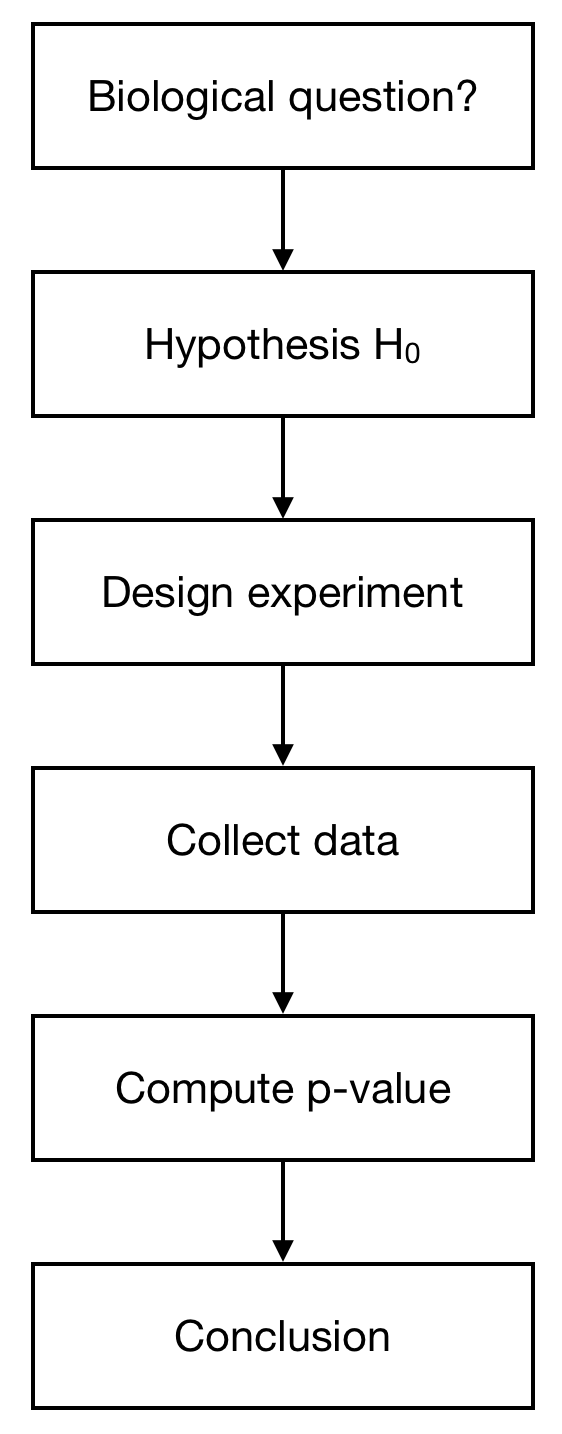
\includegraphics[height=0.5\textheight]{main_figures/intro/fisher_paradigm.png}
    \caption{Fisher's paradigm.}
    \label{fig:fisher}
\end{subfigure}
\hfill
\begin{subfigure}{0.65\textwidth}
    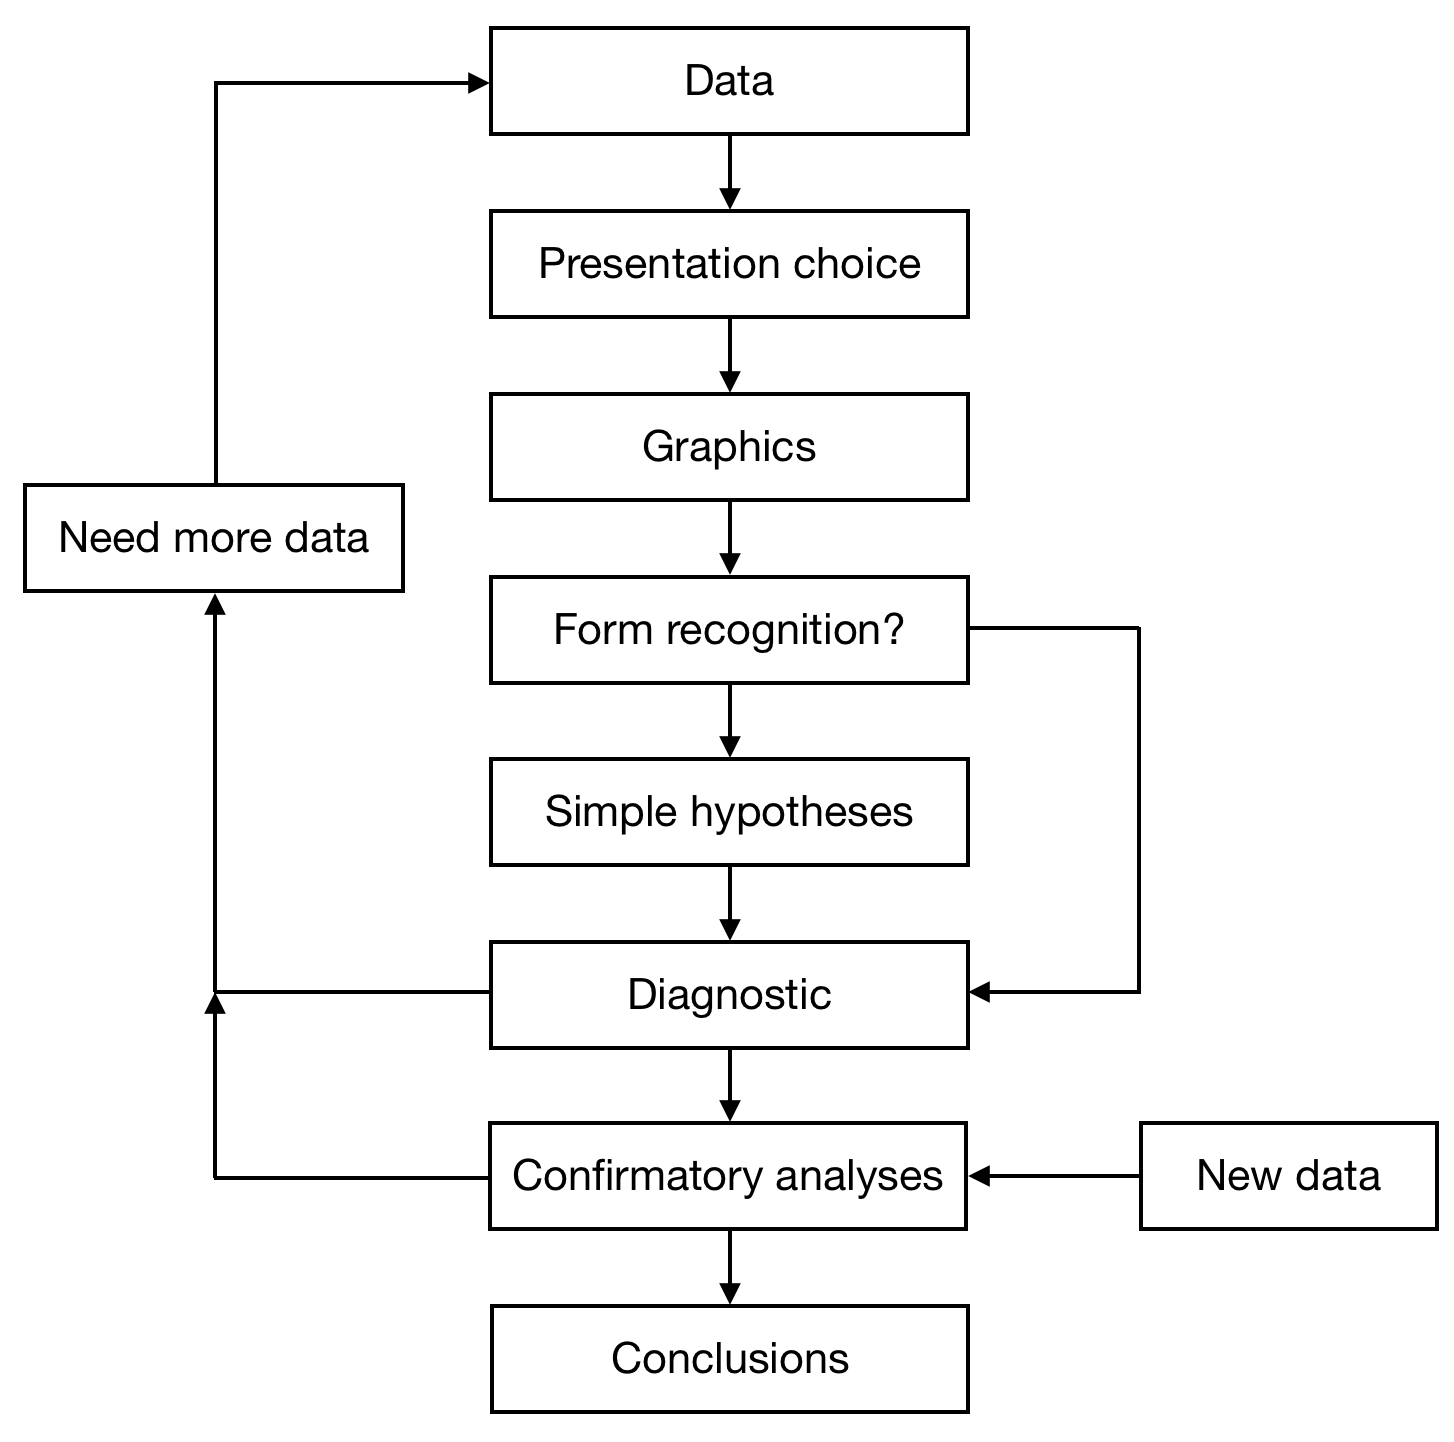
\includegraphics[height=0.5\textheight]{main_figures/intro/tukey_paradigm.png}
    \caption{Tukey's paradigm.}
    \label{fig:tukey}
\end{subfigure}
\caption{\textbf{Contrasting Fisher's paradigm with Tukey's paradigm in biology.} Fisher's paradigm (left) takes a sequential approach to data analysis, beginning with a well-defined question and strong assumptions. Tukey's paradigm (right) is iterative, beginning with the data, emphasizing exploratory analysis through visualization, and complemented by confirmatory analyses that are robust and do not rely on complex assumptions\citep{holmes_modern_2019}.}
\label{fig:paradigms}
\end{figure}

Writing in 1980, Tukey emphasized that science neither begins with a tidy question nor ends with a tidy answer\citep{tukey_we_1980}. This is especially true in modern biology. Statistical questions from the 1930s typically had a few parameters $p$ with a manageable sample size $N$ (where $N > p$), and the people posing questions were involved in data collection. Today we sit at the opposite extreme; it is not unusual for data to have $p >> N$ with the two values differing by orders of magnitude. When studying a biobank, we may have several thousand individuals and several hundred thousand genetic markers. Generally, the people investigating data have not collected it. These factors make Tukey's paradigm much better suited to our analytical needs\citep{holmes_modern_2019}. 

\subsection{Dimensionality reduction}

In Figure~\ref{fig:tukey}, the iterative process includes presentation choices, graphics, and form recognition. This provokes a natural question: what approaches ought we use here? With genomic data comes the ``curse of dimensionality'': though we have many dimensions to our data, the signal is sparse and many methods are computationally intractable. This motivates dimensionality reduction---we wish to reduce our data to a relatively low number of dimensions, ideally preserving important characteristics of the data. Given a satisfactory representation of the data set, we can visualize it.

\subsubsection{Principal component analysis}
Principal components analysis (PCA) is a non-parametric linear transformation that projects data onto a series of orthogonal axes based on a linear combination of the original data. The axes are generated and ordered according to their eigenvalues, and the ratio of each axis' corresponding eigenvalue to the sum of all eigenvalues represents the variance explained by that axis. PCA fits an ellipsoid around the data in high dimensions and the axes of that ellipsoid are the principal components. By only selecting the largest axes---corresponding to the most explained variance --- we can reduce the dimensionality of our data while preserving significant explanatory value. We can also interpret our dimensionally reduced data in terms of how much of the overall variance it explains. Principal components are calculated through eigendecomposition of the covariance matrix; a derivation for genotype data is given in \hyperref[appendix:AppendixA]{Appendix~A}. A detailed examination of PCA in the context of population genetics can be found in \citep{mcvean_genealogical_2009}. 

PCA has seen wide application in population genetics. The top PCs often reflect isolation-by-distance and are used for visualization (e.g. within Europe\citep{novembre2008europe}). However, using them for visualization requires selecting which components to examine and is limited to $2$ or $3$ dimensions; if there is signal beyond the first few PCs, it may go unnoticed. We expand on this in \hyperref[chap:chapter1]{Chapter~1}.

They are also used to correct for population structure in genome-wide association studies (GWAS) by their inclusion as covariates in models\cite{price_principal_2006}. There are varying rules-of-thumb on how many PCs to include in a model, such as using the top $10$, looking for an ``elbow'' in the scree plot, or testing for eigenvalue significance in the Wishart distribution; however, these are merely conventions. We explore the impact of PC adjustment for phenotypes in biobanks in \hyperref[chap:chapter3]{Chapter~3}. 

\subsection{Topological data analysis}

% Note to self: Rewrite this in terms of popgen challenges
% can maybe get philosophical here
We are often interested in learning about our data in to understand its large-scale structure, e.g., identifying different cell types or related individuals. Though we have some definitions of distances, we are interested in notions of \textit{similarity} or \textit{nearness}. Topology provides the mathematical machinery for ideas rooted in qualitative geometry\citep{carlsson_topology_2009}. Topological data analysis (TDA) is a set of statistical methods that uses ideas of shape and connectivity to study data\citep{wasserman_topological_2018}. We will focus on applications of manifold learning, non-linear dimensionality reduction, and density clustering.

TDA assumes that we observe a sample $X_1, \dots, X_n \sim P$ with $P$ supported on some set $\supp(P) = \mathcal{X} \subseteq \mathbb{R}^d$. 
In the simplest case of manifold learning, we suppose that $P$ is actually supported on some set $S$ with dimension $r$, where $r < d$ and $S$ is a smooth and compact manifold, and we may estimate $S$. PCA is a special case of linear manifold learning where data are assumed to lie on or near an affine subspace\citep{wasserman_topological_2018}. In cases where there is local nonlinear structure (such as clustering), nonlinear methods of manifold learning are more useful\cite{izenman_introduction_2012}.

In population genetics, we observe samples from, e.g., the distributions of genotypes.

\subsection{\texorpdfstring{$\mathbf{t}$}{f}-distributed stochastic neighbour embedding}
% the {f} here doesn't do anything, but we need a text character for compilation

$t$-distributed stochastic neighbour embedding ($t$-SNE) is a method of manifold learning used for visualization that was developed in 2008\citep{maaten_visualizing_2008}. By then, several methods existed to approximate the local structure of manifolds, but they suffered from the ``crowding problem''---in an attempt to preserve local distances between points, many of them are crunched together, eliminating the gaps between clusters. $t$-SNE addressed this by introducing a repulsion force between points, modelling pairwise distances between points $i$ and $j$ as a $t$-distributed random variable with $1$ degree of freedom (equivalent to a Cauchy distribution). The distances are modelled as probabilities:

$$q_{ij} = \frac{(1 + ||y_{i} - y_{j}||^{2})^{-1}}{\sum_{k \neq l}(1 + ||y_{k} - y_{l}||^{2})^{-1}}$$

This choice was largely ad-hoc and was later found to work because it optimized structure at the local scale (i.e. within clusters) as well as causing points to repel each other (i.e. causing clusters to separate)\citep{carreira-perpinan_elastic_2010}. This repulsion allowed $t$-SNE and related methods to preserve topology\citep{wasserman_topological_2018}. Because $t$-SNE can only reduce data to $2$ or $3$ dimensions, it was not recommended as a general purpose dimensionality reduction algorithm\citep{maaten_visualizing_2008}. It saw considerable use in visualization in single-cell genomics\citep{kobak_art_2019}, but its application in population genetics was limited (e.g. \citep{li_application_2017}). We provide details on $t$-SNE's performance in population genetics in \hyperref[chap:chapter1]{Chapter~1}.

\subsection{Uniform manifold approximation and projection}

Uniform manifold approximation and projection (UMAP) is a general purpose dimensionality reduction method rooted in algebraic topology and Riemannian geometry that was introduced in 2018\citep{mcinnes_umap_2020}. Unlike the more heuristic approach of $t$-SNE, the motivation behind UMAP is to represent the high-dimensional topology of data in low dimensional space. We will briefly outline the intuition underlying UMAP; details on the topology and theoretical justifications are available in \citep{mcinnes_umap_2020}, with a more applied explanation available in online documentation\citep{mcinnes_umapdoc_2018}.

We assume our data $X = \{X_{1}, \dots, X_{n}\}$ lay on some manifold and are uniformly distributed. For this assumption to hold, each point $X_{i}$ has its own custom distance, defined as the normalized distance to its $k\textsuperscript{th}$ nearest neighbour; thus, each $X_{i}$ has its own metric space, and is the centre of a unit ball that extends to the $k\textsuperscript{th}$ nearest neighbour. If we represent this as a graph, each $X_i$ is a point with edges to its $k$ neighbours, where the distances represent the edge weights. If we represent this as a simplicial complex, a point is a $0$-simplex and an edge is a $1$-simplex; according to theory, this simplicial complex forms an open cover of the underlying topological space. As the edge weights are between $0$ and $1$, we may also interpret the values as the belongingness to an open cover rather than a binary ``yes'' or ``no'' value---a fuzzy topological cover. To harmonize the respective edge weights $a, b$ from points $X_{a}$ to $X_{b}$ (since each point has its own local metric), UMAP defines the combined weight as $a + b - a \times b$, interpreted as the probability that an edge weight between $X_{a}$ and $X_{b}$ exists. The final high-dimensional product is a fuzzy simplicial complex, which can be represented as a weighted graph, and is a fuzzy topological representation of the data.

For the low-dimensional representation, we carry out the same process of building a fuzzy topological representation. However, rather than using a locally-varying metric, we assume that our data will lay on a low-dimensional Euclidean space, and we specify a minimum distance we wish to have between our points in this space. The algorithm then minimizes the cross-entropy function between the high- and low-dimensional representations. If $E$ is the set of all possible $1$-simplices, $w_{h}(e)$ is the weight of edge $e$ in the high-dimensional space and $w_{l}(e)$ the low-dimensional space, we minimize:

$$ \sum_{e \in E} w_{h}(e) \log{\left(\frac{w_{h}(e)}{w_{l}(e)}\right)} + (1 - w_{h}(e)) \log{\left(\frac{1 - w_{h}(e)}{1 - w_{l}(e)}\right)} $$

Though the machinery seems roundabout in its derivation, it allows for reduction of data to an arbitrary number of dimensions and for topological interpretations. The value of $k$ defines the scale of the topology we wish to approximate, with lower values being more local and finer-scale and higher values approximating broader manifold structure. Each chapter of this thesis discusses the uses and parametrizations of UMAP in population genetics: briefly, lower values of $k$ approximate closer relationships, e.g., at a structure as fine-scale as families; higher values of minimum distance facilitate visualization, while lower values facilitate algorithmic cluster detection.

UMAP is the core method of this thesis. In \hyperref[chap:chapter1]{Chapter~1}, we use UMAP in population genetics for the first time, exploring its potential applications thoroughly and compare it to PCA and t-SNE. Having been quickly adopted after our publication, in \hyperref[chap:chapter2]{Chapter~2}, we review its uses in the field and discuss different data inputs and parametrizations. In \hyperref[chap:chapter3]{Chapter~3}, we introduce the use of UMAP for topological stratification of complex biobank data by using it to pre-process data for clustering rather than simply visualization.

``Is it possible to derive low dimensional embedding methods that explicitly preserve topological features of the data? This is an interesting open question.''\citep{wasserman_topological_2018}

\subsection{Visualization}

% some principles of visualization?

% unsupervised learning?

% clustering in popgen?

%\subsection{HDBSCAN(\texorpdfstring{$\hat{\epsilon}$}{f})}
% the {f} here doesn't do anything, but we need a text character for compilation

\citep{mcinnes_accelerated_2017}

\section{Data}

This research makes use of data from four biobanks. We focus on genotype data coded as the number of non-reference alleles. Given a set of $L$ SNPs for $N$ individuals, the genotype matrix $G$ is:

%$$
%G = \begin{bmatrix} 
%    g_{11} & g_{12} & \dots g_{1L} \\
%    \vdots & \ddots & \\
%    g_{N1} &        & g_{NL} 
%    \end{bmatrix}
%    
%\text{ where } g_{ij}\text{ is the number of non-reference alleles for individual } i \text{ at locus } j.
%$$

\subsection{The 1000 Genomes Project}

The 1000 Genomes Project (1KGP) is a publicly available data set of genetic data sampled from many populations from around the world\citep{global_2015}. We used $3,450$ genotypes from the Affy 6.0 platform sampled from $26$  populations. The populations sizes are roughly similar, with between $104$ to $183$ in each group.

\subsection{CARTaGENE}

CARTaGENE (CaG) is a cohort of residents of Qu\'{e}bec with genotype data for $29,337$ participants, who were recruited using registration data from the R\'{e}gie de l’assurance maladie du Qu\'{e}bec (RAMQ), the provincial health authority\citep{awadalla_cohort_2013}. In addition to genetic data, it contains questionnaire health data and demographic information such as country of birth and ethnicity.

\subsection{Health and Retirement Study}

The Health and Retirement Study (HRS) is a cohort of retired American individuals\citep{juster_overview_1995}. We used genotype data from 12,454 individuals from the Health and Retirement Study (HRS), genotyped on the Illumina Human Omni 2.5M platform. The database contains basic demographic data such as age, US Census Bureau region of birth, and race.

\subsection{UK biobank}

The UK biobank (UKB) is a cohort of individuals living in the United Kingdom who were recruited by inviting those registered with the National Health Service (NHS)\citep{sudlow_uk_2015}. It contains the genotypes from $488,377$ participants as well as detailed health data, phenotypic measures, geographic coordinates, and sociodemographic information such as ethnic background.

%\section{Methods}

%\subsection{PCA}

%\subsection{UMAP}

%\subsection{Genomic tools}
\printbibliography[heading=subbibintoc]
\end{refsection}

%%%%%%%%%%%%%%%%%%%
%
% MANUSCRIPT CHAPTERS
%
%%%%%%%%%%%%%%%%%%%

\part{Original contributions to knowledge}
\label{part:manuscripts}

\begin{refsection}
\unchapter{UMAP reveals cryptic population structure and phenotype heterogeneity in large genomic cohorts}
\chapter*{UMAP reveals cryptic population structure and phenotype heterogeneity in large genomic cohorts}
\label{chap:chapter1}
\setcounter{section}{-1}

\section{Preface}

In Chapter 1, we apply UMAP to population genetic data for the first time. Until this time, dimensionality reduction in population genetics was largely limited to PCA, with the occasional foray into methods like t-SNE. We provide an in-depth analysis and comparison of PCA, t-SNE, and UMAP on genotype data from three biobanks: the 1KGP, the HRS, and the UKB.

We explore a variety of visualization methods and illustrate the relative strengths of UMAP as well as its limitations compared to other methods. We use UMAP to reduce our data to $2$ dimensions and uncover fine-scale population structure in each of our data sets and colour it with sociodemographic data, geographic coordinates, phenotype distributions, admixture estimates, and other variables to reveal intricate patterns. We use UMAP to reduce our data to $3$ dimensions and translate this from $(x,y,z)$ coordinates to $(R,G,B)$ values to show how to use topological data analysis to reveal spatial gradients in population structure.

This manuscript became the basis of several UMAP analyses by other researchers in a wide variety of contexts. It is now standard for new biobanks to publish a UMAP plot of their population structure. This manuscript was released as a preprint on \textit{BioRxiv} in 2018 and published in \textit{PLoS Genetics} in 2019.

\section{Abstract}

Human populations feature both discrete and continuous patterns of variation. Current analysis approaches struggle to jointly identify these patterns because of modelling assumptions, mathematical constraints, or numerical challenges. Here we apply uniform manifold approximation and projection (UMAP), a non-linear dimension reduction tool, to three well-studied genotype datasets and discover overlooked subpopulations within the American Hispanic population, fine-scale relationships between geography, genotypes, and phenotypes in the UK population, and cryptic structure in the Thousand Genomes Project data. This approach is well-suited to the influx of large and diverse data and opens new lines of inquiry in population-scale datasets.

\section{Author summary}

The demographic history of human populations features varying geographic and social barriers to mating. Over time, these barriers have led to varying levels of genetic relatedness among individuals.  This population structure is informative about human history, and can have a significant impact on studies of medical genetics. Because population structure depends on myriad demographic, ecological, and social forces, a priori visualization is useful to identify subtle patterns of population structure. We use a dimension reduction method---UMAP---to visualize population structure in three genomic datasets and find previously unobserved patterns, revealing fine-scale population structure and illustrating differences between groups in traits such as white blood cell count, height, and FEV1, a measure of lung function. Using UMAP is computationally efficient and can identify fine-scale population structure in large population datasets. We find it particularly useful to reveal phenotypic variation among genetically related populations, and recommend it is a complement  to principal component analysis in primary data visualization. 

\section{Introduction}
Questions in medicine, anthropology, and related fields hinge on interpreting the deluge of genomic data provided by modern high-throughput sequencing technologies. Because genomic datasets are high-dimensional, their interpretation requires statistical methods that can comprehensively condense information in a manner that is understandable to researchers and minimizes the amount of data that is sacrificed. Both model-based and model-agnostic approaches to summarize data have played important roles in shaping our understanding of the evolution of our species (e.g., \citep{lawson2012inference, novembre2016recent, spence2018inference, eigen2006, Hellenthal747}).

Here we will focus on nonparametric approaches to visualize relatedness patterns among individuals within populations. If we consider unphased single nucleotide polymorphism (SNP) data, an individual genome can be represented as a sequence of integers corresponding to the number of copies of the alleles carried by the individual at each of the $L$ SNPs for which genotypes are available, with $L$ ranging from hundreds of thousands to hundreds of millions. Since each individual is represented as an $L$-dimensional vector, dimension reduction methods are needed to visualize the data.

Principal component analysis (PCA) is often the first dimensional reduction tool used for genomic data. It identifies and ranks directions in genotype space that explain most-to-least variance among individuals. Positions of individuals along directions of highest variance can then be used to summarize individual genotypes. PCA coordinates have natural genealogical interpretations in terms of expected times to a most recent common ancestor (TMRCA) \citep{mcvean2009genealogical}, and are used empirically to reveal admixture \citep{brisbin2012pcadmix}, continuous isolation-by-distance \citep{novembre2008europe, nelson2008population}, as well as technical artefacts. PCA coordinates are particularly well-suited to correct for population structure in GWAS\citep{eigen2006}.

The amount of information encoded in the highest-variance PCs increases slowly with sample size, so researchers typically examine multiple two-dimensional projections to lower-variance PCs to explore data. In this process, finer features of the data may be hidden by the projections or hard to interpret. To display finer features of the data in a two dimensional figure, we can use non-linear transformations that emphasize the local structure of the data. A popular method for such visualization is t-distributed stochastic neighbour embedding (t-SNE)\citep{maaten2008visualizing}. t-SNE has been used before to visualize SNPs\citep{platzer2013visualization}. Using data from the 1000 Genomes Project (1KGP)\citep{10002015global}, it groups individuals corresponding roughly to their continent of origin, with smaller ethnic sub-groups visible within the larger continental clusters\citep{li2017tsne}. However, t-SNE struggles with very large datasets, when a large number of locally optimal configurations make convergence to a globally satisfying solution difficult.

Uniform Manifold Approximation and Projection (UMAP) is a dimension reduction technique designed to model and preserve the high-dimensional topology of data points in the low-dimensional space\citep{2018arXivUMAP}. With genotype data, UMAP creates a neighbourhood around each individual's genetic coordinates and identifies a pre-selected number of neighbours to build high-dimensional manifolds. The end result is a patchwork of low-dimensional representations of neighbourhoods that groups genetically similar individuals together on a local scale while better preserving long-range topological connections to more distantly related individuals. The method has been successfully applied to single-cell RNA sequencing datasets \citep{umap2018singlecell}.

Non-linear dimension reduction methods tend to be computationally intensive. A common practice to reduce this burden is to first apply PCA to data, and perform dimensional reduction on data projected to leading principal components (PCs). In addition to being computationally advantageous, this discards noise that can confound non-linear approaches: population structure arising from $n$ isolated randomly-mating demes can be described by the leading $n-1$ PCs, with the following PCs describing stochastic variation in relatedness~\citep{eigen2006}. Selecting the leading PCs therefore has potential to extract meaningful population structure while filtering out stochastic noise. We explore different strategies to pre-process the data and investigate discrete and continuous population structure patterns present in large datasets of human genotypes: the 1KGP, the Health and Retirement Study (HRS)\citep{juster1995overview}, and the UK BioBank (UKBB)\citep{sudlow2015uk}, and compare UMAP's performance to t-SNE.  

\section{Results}
\subsection{Fine-scale visualization of the 1KGP dataset}

\begin{figure}[!ht]
    \centering
    
\includegraphics[width=0.7\textwidth]{placeholder.png}
    \caption[Four methods of dimension reduction of 1KGP genotype data]{\textbf{Four methods of dimension reduction of 1KGP genotype data with population labels.} \textbf{(A)} PCA maps individuals in a triangle with vertices corresponding to African, Asian, and European continental ancestry. Discarding lower-variance PCs leads to overlap of populations with no close affinity, such as Central and South American populations with South Asians. \textbf{(B)} t-SNE forms groups corresponding to continents, with some overlap between European and Central and South American people. Smaller subgroups are visible within continental clusters. The cloud of peripheral points results from the method's poor convergence. \textbf{(C)} UMAP forms distinct clusters related to continent with clearly defined subgroups. Japanese, Finnish, Luhya, and some Punjabi and Telugu populations form separate clusters consistent with their population history\citep{10002015global}. \textbf{(D)} UMAP on the first 15 principal components forms fine-scale clusters for individual populations. Groups closely related by ancestry or geography, such as African Caribbean/African American, Spanish/Italian, and Kinh/Dai populations cluster together. Results using t-SNE on principal components are presented in \ref{fig:supp_megamontage_pc2_9}. Axes in UMAP and t-SNE are arbitrary. Since the algorithms prioritize local distances, long distances between clusters are not meaningful.}
    \label{fig:fig1}
\end{figure}

The 1KGP contains genotype data of 3,450 individuals from 26 relatively distinct labeled populations\citep{10002015global}. Fig~\ref{fig:fig1} shows visualizations using PCA, t-SNE, UMAP, and UMAP with PCA pre-processing. Using UMAP and t-SNE on the genotype data presents clusters that are roughly grouped by continent, with UMAP showing a clear hierarchy of population and continental clusters, whereas t-SNE fails to assign many individuals to population clusters. Using either method on the top principal components leads to distinct population clusters and less defined continental structure. Adding more components results in progressively finer clusters until approximately 20 populations appear using 15 components; adding further components converges to results similar to using the entire genotype data (see \ref{fig:supp_megamontage_pc2_9}, \ref{fig:supp_megamontage_pc10_50}, and \ref{fig:supp_montage_1kgp_converge}). To investigate the population information contained in low-variance PCs, we performed UMAP on data projected onto PCs 100 to 3450 (i.e., without information about the leading 99 PCs). \nameref{fig:supp_1kgp_3350} shows that population structure is still clearly visible.

Focusing on UMAP with the leading 15 principal components (\ref{fig:fig1}D), several population clusters reflect shared ancestries. British individuals from England and Scotland form a cluster mixed with those from Utah who claim Northern and Western European ancestry. Toscani and Iberian individuals form a cluster reflecting their Mediterranean heritage. African Americans in the Southwest US, African Caribbean individuals in Barbados, and some Puerto Ricans also form a cluster. Three East Asian clusters appear: one is largely Han and Southern Han individuals, another is comprised of the Chinese Dai in southern China and the Kinh from Vietnam, and the third is the Japanese population. Other clusters are comprised of Colombians and Peruvians, the Esan and Yoruba populations of Nigeria, and several South Asian populations. 

Within population clusters, family members were projected near each other within broader population groups. When UMAP was parameterized to use only 5 nearest neighbours, however, families often formed distinct clusters (\ref{fig:supp_1kgp_families}): Using few neighbours to build a manifold emphasizes closer relatedness.

\newpage

\section{Supporting information}

\begin{figure}[ht]
    \centering
    \begin{subfigure}{\textwidth}
    %\includegraphics[width=\textwidth]{images/megamontage_PC2_9.pdf}
    
\includegraphics[width=0.7\textwidth]{placeholder.png}
    \end{subfigure}
    \caption[Montage of t-SNE and UMAP on up to 9 PCs of 1KGP data]{\textbf{Montage of t-SNE and UMAP on up to 9 PCs of 1KGP data.} UMAP (left two columns) and t-SNE (right two columns) applied to the top principal components of the 1KGP labelled by the number of components used. Adding more components results in progressively finer population clusters using both methods.}
    \label{fig:supp_megamontage_pc2_9}  
\end{figure}

\newpage

\begin{figure}[ht]
    \centering
    \begin{subfigure}{0.95\textwidth}
    %\includegraphics[width=0.95\textwidth]{images/megamontage_PC10_50.pdf}
    
\includegraphics[width=0.7\textwidth]{placeholder.png}
    \end{subfigure}
    \caption[Montage of t-SNE and UMAP on 10 to 50 PCs of 1KGP data]{\textbf{Montage of t-SNE and UMAP on 10 to 50 PCs of 1KGP data.} UMAP (left two columns) and t-SNE (right two columns) applied to the top principal components of the 1KGP labelled by the number of components used. Results are similar until approximately 11 components, where t-SNE breaks apart clusters of South Asian (in green) and Central and South American populations (in pink) while UMAP preserves them. At approximately 30 components populations begin to drift together with UMAP and disperse with t-SNE.}
    \label{fig:supp_megamontage_pc10_50}
\end{figure}

\newpage

\begin{figure}[ht]
    \centering
    \begin{subfigure}{0.95\textwidth}
    %\includegraphics[width=0.95\textwidth]{images/montage_1KGP_umap_convergence_resize.jpeg}
    
\includegraphics[width=0.7\textwidth]{placeholder.png}
    \end{subfigure}
    \caption[Montage of UMAP on progressively more PCs of 1KGP data]{\textbf{Montage of UMAP on progressively more PCs of 1KGP data.} UMAP applied to the first few hundred principal components of the 1KGP data with the amount of variance explained in parentheses. As more components are added, the figure begins to resemble that of UMAP carried out on the full genotype dataset.}
    \label{fig:supp_montage_1kgp_converge}
\end{figure}

\newpage

\begin{figure}[ht]
    \centering
    \begin{subfigure}{0.95\textwidth}
    %\includegraphics[width=0.95\textwidth]{images/1KGP_UMAP_PCS100_PCE3450_NC2_NN15_MD05_201944185843.jpeg}
    
\includegraphics[width=0.7\textwidth]{placeholder.png}
    \end{subfigure}
    \caption[UMAP on PCs 100 to 3350 of 1KGP data]{\textbf{UMAP on PCs 100 to 3350 of 1KGP data.} UMAP applied the last 3350 principal components of the 1KGP, which explain 78.7\% of the variation. The colour scheme is the same as in \ref{fig:fig1}.}
    \label{fig:supp_1kgp_3350}
\end{figure}

\newpage

\begin{figure}[ht]
    \centering
    \begin{subfigure}{\textwidth}
    %\includegraphics[width=0.52\textwidth]{images/1KGP_UMAP_PC15_families.png}
    
\includegraphics[width=0.7\textwidth]{placeholder.png}
    \end{subfigure}
    \caption[Number of neighbours and families forming disjoint clusters]{\textbf{Number of neighbours and families forming disjoint clusters.} UMAP applied to the first 15 principal components of the 1KGP, with the number of neighbours set to 5 (top) and 15 (bottom). Six members of one Southern Han Chinese family are highlighted: HG00656 (grandfather), HG00657 (grandmother), HG00658 (uncle, mother's brother), HG00701 (mother), HG00702 (father), HG00703 (child). When using UMAP with five neighbours, the father (in blue) is projected to the cluster of the Southern Han Chinese population while the rest of the family members (in red) form their own disjoint cluster. Using 15 neighbours, the family still clusters together, but as part of the Southern Han Chinese population rather than a separate cluster.}
    \label{fig:supp_1kgp_families}
\end{figure}

\newpage

\begin{figure}[ht]
    \centering
    \begin{subfigure}{0.95\textwidth}
    %\includegraphics[width=0.75\textwidth]{images/HRS_1000G_NP1_UMAP_PC10_NC2_NN15_MD05_pca_1kgp_onto_hrs_umap_1kgp_onto_hrs_2018112221116_race_hisp_mex_labels.pdf}
    
\includegraphics[width=0.7\textwidth]{placeholder.png}
    \end{subfigure}
    \caption[UMAP on HRS data coloured by ethnicity]{\textbf{UMAP on HRS data coloured by ethnicity.} UMAP applied to the first 10 principal components of HRS data. Points coloured by self-identified race, Hispanic status, and Mexican-American status. The cluster on the left is mostly people who identify as neither Black nor White and were born outside the contiguous United States or in the Pacific census region. Clustering with the 1KGP data places them with Asian-identified populations. BNH, Black (not Hispanic); BHO, Black (Hispanic, Other); WNH, White (not Hispanic); WHM, White (Hispanic, Mexican-American); WHO, White Hispanic (Other); ONH, Other (not Hispanic); OHM, Other (Hispanic, Mexican-American); OHO, Other (Hispanic, Other).}
    \label{fig:supp_umap_hrs_eth}
\end{figure}

\newpage

\begin{figure}
\centering
   %\includegraphics[width=0.6\linewidth]{images/HRS_1000G_NP1_UMAP_PC10_NC2_NN15_MD05_pca_1kgp_onto_hrs_umap_1kgp_onto_hrs_2018112221116_admix.jpeg}
    
\includegraphics[width=0.7\textwidth]{placeholder.png}
   \caption[UMAP on HRS data coloured by admixture]{\textbf{UMAP on HRS data coloured by admixture.} UMAP on the first 10 principal components of HRS data. colouring individuals by estimated admixture from three ancestral populations reveals considerable diversity in the Hispanic population. This projection coloured by self-identified race and Hispanic status is presented in \ref{fig:supp_umap_hrs_eth}. Admixture proportions for each individual were estimated in (Baharian 2016) by assuming ancestral African, Asian, and European populations using RFMIX. We have scaled each of the three proportions to values between 0 and 255 (with 100\% corresponding to 255), to colour individual points by their estimated admixture represented by RGB where red, green, and blue respectively correspond to African, European, and Asian/Native American ancestry. An alternate colouring is provided in \ref{fig:umap_hrs_admix_alt}.}
    \label{fig:umap_hrs_admix}
\end{figure}

\newpage

\begin{figure}[ht]
    \centering
    \begin{subfigure}{\textwidth}
    %\includegraphics[width=0.9\textwidth]{images/HRS_1000G_NP1_UMAP_PC10_NC2_NN15_MD05_pca_1kgp_onto_hrs_umap_1kgp_onto_hrs_2018112221116_born.jpeg}
    
\includegraphics[width=0.7\textwidth]{placeholder.png}
    \end{subfigure}
    \caption[UMAP on HRS data coloured by birth region]{\textbf{UMAP on HRS data coloured by birth region.} UMAP on the top 10 principal components of the HRS dataset, coloured by Census Bureau birth region. Each colour represents one of the 10 birth regions. There is no obvious pattern in the clusters of majority ``White Not Hispanic'' individuals.}
    \label{fig:supp_hrs_born}
\end{figure}

\newpage

\begin{figure}[ht]
    \centering
    \begin{subfigure}{\textwidth}
    %\includegraphics[width=\textwidth]{images/HRS_1000G_NP1_UMAP_PC10_NC2_NN15_MD05_pca_1kgp_onto_hrs_umap_1kgp_onto_hrs_2018112221116_custom_label.pdf}
    
\includegraphics[width=0.7\textwidth]{placeholder.png}
    \end{subfigure}
    \caption[UMAP on HRS data with 1KGP data overlaid]{\textbf{UMAP on HRS data with 1KGP data overlaid.} UMAP on the top 10 principal components of the HRS data, with 1KGP data projected onto the embedding. Individuals from the HRS are grey. British (GBR) and other European (CEU) individuals are scattered throughout the ``White Not Hispanic'' clusters. Finns (FIN) form clear groupings. Spanish (IBS) and Italian (TSI) individuals cluster near the Hispanic grouping. There are sub-groups in the Hispanic cluster formed of Puerto Ricans (PUR), Colombians (CLM), Mexicans (MXL), and Peruvians (PEL). Populations with African ancestry (AFR) appear with Black individuals. East Asian (EAS) populations comprising Chinese, Kinh, and Japanese individuals cluster together with what appears in \ref{fig:umap_hrs_admix} as a population of mostly Asian ancestry. South Asian (SAS) populations with Indian, Pakistani, and Sri Lankan ancestry cluster in a separate area. One ``White Not Hispanic'' cluster at the bottom does not cluster with any 1KGP populations.}
    \label{fig:supp_hrs_1kgp_projected}
\end{figure}

\newpage

\begin{figure}[ht]
    \centering
    \begin{subfigure}{\textwidth}
    %\includegraphics[width=\textwidth]{images/HRS_PCGRID_8.pdf}
    
\includegraphics[width=0.7\textwidth]{placeholder.png}
    \end{subfigure}
    \caption[Pairwise plots of PCs of Hispanic HRS data]{\textbf{Pairwise plots of PCs of Hispanic HRS data.} Pairwise plots of the first 8 principal components of the Hispanic subset of the HRS. Those born in the Mountain region are coloured green.}
    \label{fig:supp_hrs_hisp_grid}
\end{figure}

\newpage

\begin{figure}[ht]
    \centering
    \begin{subfigure}{\textwidth}
    %\includegraphics[width=0.7\textwidth]{images/HRS_1000G_NP1_UMAP_PC7_NC2_NN15_MD05_pca_hrshisp_added1kgp_2018115153245_admix.jpeg}
    
\includegraphics[width=0.7\textwidth]{placeholder.png}
    \end{subfigure}
    \caption[UMAP on Hispanic HRS data coloured by admixture]{\textbf{UMAP on Hispanic HRS data coloured by admixture.} UMAP of the first 7 principal components of the Hispanic population of the HRS, coloured by estimated admixture proportions. Admixture proportions for each individual were estimated in (Baharian, 2016) by assuming ancestral African, Asian, and European populations using RFMIX. We have scaled each of the three proportions to values between 0 and 255 (with 100\% corresponding to 255), to colour individual points by their estimated admixture represented by RGB where red, green, and blue respectively correspond to African, European, and Asian/Native American ancestry. An alternate colouring is provided in \ref{fig:supp_umap_hrs_hisp_admix_alt}.}
    \label{fig:supp_umap_hrs_hisp_admix}
\end{figure}

\newpage

\begin{figure}[ht]
    \centering
    \begin{subfigure}{\textwidth}
    %\includegraphics[width=0.8\textwidth]{images/HRS_1000G_NP1_UMAP_PC7_NC2_NN15_MD05_pca_hrshisp_added1kgp_2018115153245_1kgp_hisp_birthonly.jpeg}
    
\includegraphics[width=0.7\textwidth]{placeholder.png}
    \end{subfigure}
    \caption[UMAP on Hispanic HRS data coloured by birth region]{\textbf{UMAP on Hispanic HRS data coloured by birth region.} UMAP of the first 7 principal components of the Hispanic population of the HRS, coloured region of birth.}
    \label{fig:supp_umap_hrs_hisp_birth}
\end{figure}

\newpage

\begin{figure}[ht]
    \centering
    \begin{subfigure}{\textwidth}
    %\includegraphics[width=0.8\textwidth]{images/Asthma_FullAsian_PC_QC_new_UMAP_PC5_NC2_NN15_MD05_201931173256.jpeg}
    
\includegraphics[width=0.7\textwidth]{placeholder.png}
    \end{subfigure}
    \caption[UMAP on Asian UKBB data coloured by self-identified ethnicity]{\textbf{UMAP on Asian UKBB data coloured by self-identified ethnicity.} UMAP of the first 8 principal components of the Asian population in the UKBB coloured by self-identified ethnicity. This is an alternate colouring of \ref{fig:fig2}B.}
    \label{fig:supp_umap_ukbb_asian_eth}
\end{figure}

\newpage

\begin{figure}[ht]
    \centering
    \begin{subfigure}{0.8\textwidth}
    %\includegraphics[width=\textwidth]{images/UKBB_UMAP_PC10_NN15_MD05_eth_cob_resized.jpeg}
    
\includegraphics[width=0.7\textwidth]{placeholder.png}
    \end{subfigure}
    \caption[UMAP on UKBB data with some countries of birth identified]{\textbf{UMAP on UKBB data with some countries of birth identified.} Using country of birth data, some of the larger unidentified groups from \ref{fig:fig3}B were identified as being born mostly in Japan, the Philippines, North Africa, the Middle East, and Central and South America. The large cluster of ``Any other Asian Background'' were mostly born in Sri Lanka.}
    \label{fig:supp_ukbb_cob}
\end{figure}

\newpage

\begin{figure}[ht]
    \centering
    \begin{subfigure}{0.9\textwidth}
    %\includegraphics[width=0.9\textwidth]{images/UKBB_UMAP_PC10_NN15_MD05_2018328174511_london_permuted_10nn_sd10_base1_maxdist200_2019625172227_resize.jpeg}
    
\includegraphics[width=0.7\textwidth]{placeholder.png}
    \end{subfigure}
    \caption[UMAP on UKBB data coloured by distance from London]{\textbf{UMAP on UKBB data coloured by distance from London.} UMAP on UKBB data, coloured by distance from London, with red representing those living closer to London and blue representing those living farther from London. A 200km radius extends roughly to Cardiff, and a 100km radius extends roughly to cities such as Leicester and Bath, and contains cities such as Oxford, Cambridge, and Peterborough. Data has been randomized as explained in the materials and methods section.}
    \label{fig:supp_london_distance}
\end{figure}

\newpage

\begin{figure}[ht]
    \centering
    \begin{subfigure}{0.95\textwidth}
    %\includegraphics[width=0.95\textwidth]{images/default_clean_size10_alpha60_flip.jpeg}
    
\includegraphics[width=0.7\textwidth]{placeholder.png}
    \end{subfigure}
    \caption[Montage of UMAP on top 40 PCs of UKBB data coloured by ethnicity]{\textbf{Montage of UMAP on top 40 PCs of UKBB data coloured by ethnicity.} UMAP on UKBB data, coloured by self-identified ethnic background. Images are labelled by the number of components included.}
    \label{fig:supp_montage_ukbb_eth}
\end{figure}

\newpage

\begin{figure}[ht]
    \centering
    \begin{subfigure}{0.95\textwidth}
    %\includegraphics[width=0.95\textwidth]{images/default_clean_size10_alpha60_ns.jpeg}
    
\includegraphics[width=0.7\textwidth]{placeholder.png}
    \end{subfigure}
    \caption[Montage of UMAP on top 40 PCs of UKBB data coloured by northing]{\textbf{Montage of UMAP on top 40 PCs of UKBB data coloured by northing.} UMAP on UKBB data, coloured by northing values, with more blue representing more northern coordinates and more red representing more southern coordinates. Images are labelled by the number of components included. Data has been randomized as explained in the materials and methods section.}
    \label{fig:supp_montage_ukbb_ns}
\end{figure}

\newpage

\begin{figure}[ht]
    \centering
    \begin{subfigure}{\textwidth}
    %\includegraphics[width=\textwidth]{images/default_clean_size10_alpha60_ew.jpeg}
    
\includegraphics[width=0.7\textwidth]{placeholder.png}
    \end{subfigure}
    \caption[Montage of UMAP on top 40 PCs of UKBB data coloured by easting]{\textbf{Montage of UMAP on top 40 PCs of UKBB data coloured by easting.} UMAP on UKBB data, coloured by easting values, with more yellow representing more eastern coordinates and more pink representing more western coordinates. Images are labelled by the number of components included. Data has been randomized as explained in the materials and methods section.}
    \label{fig:supp_montage_ukbb_ew}
\end{figure}

\newpage

\begin{figure}[ht]
    \centering
    \begin{subfigure}{\textwidth}
    %\includegraphics[width=\textwidth]{images/meanAsiaMap.jpg}
    
\includegraphics[width=0.7\textwidth]{placeholder.png}
    \end{subfigure}
    \caption[Map of Asia coloured by 3D UMAP coordinates of UKBB data]{\textbf{Map of Asia coloured by 3D UMAP coordinates of UKBB data.} Fig 5b, zoomed in on Asia. Geographic distribution of UMAP coordinates. Using the country of birth of individuals in the UKBB, we colour countries by the closeness in 3D UMAP space of those born there. Broad patterns of similarity appear in East Asia, South Asia, North African and the Middle East, West Africa, and South America. Differences between neighbouring countries can reflect both ancient population structure and recent differences in migration history. Evidence of migrations related to colonialism are visible with, e.g., European ancestry in South Africa and South Asian ancestry in Kenya and Tanzania. Because of the large number of White British individuals born abroad, to avoid skewing the colour scale they were not included unless they were born in the UK, Europe, Australia, Canada, or the United States, where UKBB participants already tended to have European ancestry.}
    \label{fig:supp_umap_ukbb_asia}
\end{figure}

\newpage

\begin{figure}[ht]
    \centering
    \begin{subfigure}{\textwidth}
    %\includegraphics[width=\textwidth]{images/meanCarribeanMap.jpg}
    
\includegraphics[width=0.7\textwidth]{placeholder.png}
    \end{subfigure}
    \caption[Map of Caribbean coloured by 3D UMAP coordinates of UKBB data]{\textbf{Map of Caribbean coloured by 3D UMAP coordinates of UKBB data.} Fig 5b, zoomed in on the Caribbean. Geographic distribution of UMAP coordinates. Using the country of birth of individuals in the UKBB, we colour countries by the closeness in 3D UMAP space of those born there. Broad patterns of similarity appear in East Asia, South Asia, North African and the Middle East, West Africa, and South America. Differences between neighbouring countries can reflect both ancient population structure and recent differences in migration history. Evidence of migrations related to colonialism are visible with, e.g., European ancestry in South Africa and South Asian ancestry in Kenya and Tanzania. Because of the large number of White British individuals born abroad, to avoid skewing the colour scale they were not included unless they were born in the UK, Europe, Australia, Canada, or the United States, where UKBB participants already tended to have European ancestry.}
    \label{fig:supp_umap_ukbb_car}
\end{figure}

\newpage

\begin{figure}[ht]
    \centering
    \begin{subfigure}{\textwidth}
    %\includegraphics[width=\textwidth]{images/meanEuroMap.jpg}
    
\includegraphics[width=0.7\textwidth]{placeholder.png}
    \end{subfigure}
    \caption[Map of Europe coloured by 3D UMAP coordinates of UKBB data]{\textbf{Map of Europe coloured by 3D UMAP coordinates of UKBB data.} Fig 5b, zoomed in on Europe. Geographic distribution of UMAP coordinates. Using the country of birth of individuals in the UKBB, we colour countries by the closeness in 3D UMAP space of those born there. Broad patterns of similarity appear in East Asia, South Asia, North African and the Middle East, West Africa, and South America. Differences between neighbouring countries can reflect both ancient population structure and recent differences in migration history. Evidence of migrations related to colonialism are visible with, e.g., European ancestry in South Africa and South Asian ancestry in Kenya and Tanzania. Because of the large number of White British individuals born abroad, to avoid skewing the colour scale they were not included unless they were born in the UK, Europe, Australia, Canada, or the United States, where UKBB participants already tended to have European ancestry.}
    \label{fig:supp_umap_ukbb_eur}
\end{figure}

\newpage

\begin{figure}[!htb]
    \centering
    %\includegraphics[width=0.95\columnwidth]{images/UKBB_TSNE_10PCs_DefaultPerplexity_eth.pdf}
    
\includegraphics[width=0.7\textwidth]{placeholder.png}
    \caption[t-SNE on UKBB data coloured by self-identified ethinicity]{\textbf{t-SNE on UKBB data coloured by self-identified ethinicity.} t-SNE applied to the top 10 principal components of the UKBB, coloured by ethnic background. The unbalanced populations resulted in many individuals and populations being orphaned along the periphery of the main cluster.}
    \label{fig:supp_ukbb_tsne}
\end{figure}

%%%%% UKBB phenotype plots
\begin{figure}[ht]
    \centering
    %\includegraphics[width=0.4\columnwidth]{images/UKBB_UMAP_PC10_NN15_MD05_2018328174511_201871417039_basophill_count_pct5_f.pdf}
    \includegraphics[width=0.7\textwidth]{placeholder.png}
    \caption[UMAP on UKBB data coloured by basophil count (female)]{\textbf{UMAP on UKBB data coloured by basophil count (female).} UMAP on the top 10 principal components of the UKBB coloured by basophil count (female). Data has been randomized as explained in the materials and methods section.}
    \label{fig:supp_ukbb_basophill_f}
\end{figure}

\newpage

\begin{figure}[ht]
    \centering
    %\includegraphics[width=0.4\columnwidth]{images/UKBB_UMAP_PC10_NN15_MD05_2018328174511_201871417039_basophill_count_pct5_m.pdf}
    \includegraphics[width=0.7\textwidth]{placeholder.png}
    \caption[UMAP on UKBB data coloured by basophil count (male)]{\textbf{UMAP on UKBB data coloured by basophil count (male).} UMAP on the top 10 principal components of the UKBB coloured by basophil count (male). Data has been randomized as explained in the materials and methods section.}
    \label{fig:supp_ukbb_basophill_m}
\end{figure}

\newpage

\begin{figure}[ht]
    \centering
    %\includegraphics[width=0.4\columnwidth]{images/UKBB_UMAP_PC10_NN15_MD05_2018328174511_201871417720_eosinophill_count_pct5_f.pdf}
    \includegraphics[width=0.7\textwidth]{placeholder.png}
    \caption[UMAP on UKBB data coloured by eosinphil count (female)]{\textbf{UMAP on UKBB data coloured by eosinphil count (female).} UMAP on the top 10 principal components of the UKBB coloured by eosinophil count (female). Data has been randomized as explained in the materials and methods section.}
    \label{fig:supp_ukbb_eosinophill_f}
\end{figure}

\newpage

\begin{figure}[ht]
    \centering
    %\includegraphics[width=0.4\columnwidth]{images/UKBB_UMAP_PC10_NN15_MD05_2018328174511_201871417720_eosinophill_count_pct5_m.pdf}
    \includegraphics[width=0.7\textwidth]{placeholder.png}
    \caption[UMAP on UKBB data coloured by eosinphil count (male)]{\textbf{UMAP on UKBB data coloured by eosinphil count (male).} UMAP on the top 10 principal components of the UKBB coloured by eosinophil count (male). Data has been randomized as explained in the materials and methods section.}
    \label{fig:supp_ukbb_eosinophill_m}
\end{figure}

\newpage

\begin{figure}[ht]
    \centering
    %\includegraphics[width=0.4\columnwidth]{images/UKBB_UMAP_PC10_NN15_MD05_2018328174511_201871416305_3063_0_0_pct1_f.pdf}
    \includegraphics[width=0.7\textwidth]{placeholder.png}
    \caption[UMAP on UKBB data coloured by FEV1 (female)]{\textbf{UMAP on UKBB data coloured by FEV1 (female).} UMAP on the top 10 principal components of the UKBB coloured by FEV1 (female). Data has been randomized as explained in the materials and methods section.}
    \label{fig:supp_ukbb_fev_f}
\end{figure}

\newpage

\begin{figure}[ht]
    \centering
    %\includegraphics[width=0.4\columnwidth]{images/UKBB_UMAP_PC10_NN15_MD05_2018328174511_201871416305_3063_0_0_pct1_m.pdf}
    \includegraphics[width=0.7\textwidth]{placeholder.png}
    \caption[UMAP on UKBB data coloured by FEV1 (male)]{\textbf{UMAP on UKBB data coloured by FEV1 (male).} UMAP on the top 10 principal components of the UKBB coloured by FEV1 (male). Data has been randomized as explained in the materials and methods section.}
    \label{fig:supp_ukbb_fev_m}
\end{figure}

\newpage

\begin{figure}[ht]
    \centering
    %\includegraphics[width=0.4\columnwidth]{images/UKBB_UMAP_PC10_NN15_MD05_2018328174511_2018714161841_Height_res_pct1_f.pdf}
    \includegraphics[width=0.7\textwidth]{placeholder.png}
    \caption[UMAP on UKBB data coloured by height (female)]{\textbf{UMAP on UKBB data coloured by height (female).} UMAP on the top 10 principal components of the UKBB coloured by height (female). Data has been randomized as explained in the materials and methods section.}
    \label{fig:supp_ukbb_height_f}
\end{figure}

\newpage

\begin{figure}[ht]
    \centering
    %\includegraphics[width=0.4\columnwidth]{images/UKBB_UMAP_PC10_NN15_MD05_2018328174511_2018714161841_Height_res_pct1_m.pdf}
    \includegraphics[width=0.7\textwidth]{placeholder.png}
    \caption[UMAP on UKBB data coloured by height (male)]{\textbf{UMAP on UKBB data coloured by height (male).} UMAP on the top 10 principal components of the UKBB coloured by height (male). Data has been randomized as explained in the materials and methods section.}
    \label{fig:supp_ukbb_height_m}
\end{figure}

\newpage

\begin{figure}[ht]
    \centering
    %\includegraphics[width=0.4\columnwidth]{images/UKBB_UMAP_PC10_NN15_MD05_2018328174511_201871416519_leukocyte_count_pct5_f.pdf}
    \includegraphics[width=0.7\textwidth]{placeholder.png}
    \caption[UMAP on UKBB data coloured by leukocyte count (female)]{\textbf{UMAP on UKBB data coloured by leukocyte count (female).} UMAP on the top 10 principal components of the UKBB coloured by leukocyte count (female). Data has been randomized as explained in the materials and methods section.}
    \label{fig:supp_ukbb_leukocyte_f}
\end{figure}

\newpage

\begin{figure}[ht]
    \centering
    %\includegraphics[width=0.4\columnwidth]{images/UKBB_UMAP_PC10_NN15_MD05_2018328174511_201871416519_leukocyte_count_pct5_m.pdf}
    \includegraphics[width=0.7\textwidth]{placeholder.png}
    \caption[UMAP on UKBB data coloured by leukocyte count (male)]{\textbf{UMAP on UKBB data coloured by leukocyte count (male).} UMAP on the top 10 principal components of the UKBB coloured by leukocyte count (male). Data has been randomized as explained in the materials and methods section.}
    \label{fig:supp_ukbb_leukocyte_m}
\end{figure}

\newpage

\begin{figure}[ht]
    \centering
    %\includegraphics[width=0.4\columnwidth]{images/UKBB_UMAP_PC10_NN15_MD05_2018328174511_2018714165614_neutrophill_count_pct5_f.pdf}
    \includegraphics[width=0.7\textwidth]{placeholder.png}
    \caption[UMAP on UKBB data coloured by neutrophil count (female)]{\textbf{UMAP on UKBB data coloured by neutrophil count (female).} UMAP on the top 10 principal components of the UKBB coloured by neutrophil count (female). Data has been randomized as explained in the materials and methods section.}
    \label{fig:supp_ukbb_neutrophill_f}
\end{figure}

\newpage

\begin{figure}[ht]
    \centering
    %\includegraphics[width=0.4\columnwidth]{images/UKBB_UMAP_PC10_NN15_MD05_2018328174511_2018714165614_neutrophill_count_pct5_m.pdf}
    \includegraphics[width=0.7\textwidth]{placeholder.png}
    \caption[UMAP on UKBB data coloured by neutrophil count (male)]{\textbf{UMAP on UKBB data coloured by neutrophil count (male).} UMAP on the top 10 principal components of the UKBB coloured by neutrophil count (male). Data has been randomized as explained in the materials and methods section.}
    \label{fig:supp_ukbb_neutrophill_m}
\end{figure}

\newpage

\begin{figure}[ht]
    \centering
    \begin{subfigure}{\textwidth}
    %\includegraphics[width=\textwidth]{images/female_height_boxplot_annotated.pdf}
    \includegraphics[width=0.7\textwidth]{placeholder.png}
    \end{subfigure}
    \caption[Box plots of height in the UKBB by self-identified ethnicity (female)]{\textbf{Box plots of height in the UKBB by self-identified ethnicity (female).} Height by sex and ethnic group, annotated with p-values. Asterisks indicate significant difference from the White British group with a Bonferroni correction for 12 groups.}
    \label{fig:supp_box_height_f}
\end{figure}

\newpage

\begin{figure}[ht]
    \centering
    \begin{subfigure}{\textwidth}
    %\includegraphics[width=\textwidth]{images/male_height_boxplot_annotated.pdf}
    \includegraphics[width=0.7\textwidth]{placeholder.png}
    \end{subfigure}
    \caption[Box plots of height in the UKBB by self-identified ethnicity (male)]{\textbf{Box plots of height in the UKBB by self-identified ethnicity (male).} Height by sex and ethnic group, annotated with p-values. Asterisks indicate significant difference from the White British group with a Bonferroni correction for 12 groups.}
    \label{fig:supp_box_height_m}
\end{figure}

\newpage

\begin{figure}[ht]
    \centering
    \begin{subfigure}{\textwidth}
    %\includegraphics[width=\textwidth]{images/female_fev_boxplot_annotated.pdf}
    \includegraphics[width=0.7\textwidth]{placeholder.png}
    \end{subfigure}
    \caption[Box plots of FEV1 in the UKBB by self-identified ethnicity (female)]{\textbf{Box plots of FEV1 in the UKBB by self-identified ethnicity (female).} FEV1 by sex and ethnic group, annotated with p-values. Asterisks indicate significant difference from the White British group with a Bonferroni correction for 12 groups.}
    \label{fig:supp_box_fev_f}
\end{figure}

\newpage

\begin{figure}[ht]
    \centering
    \begin{subfigure}{\textwidth}
    %\includegraphics[width=\textwidth]{images/male_fev_boxplot_annotated.pdf}
    \includegraphics[width=0.7\textwidth]{placeholder.png}
    \end{subfigure}
    \caption[Box plots of FEV1 in the UKBB by self-identified ethnicity (male)]{\textbf{Box plots of FEV1 in the UKBB by self-identified ethnicity (male).} FEV1 by sex and ethnic group, annotated with p-values. Asterisks indicate significant difference from the White British group with a Bonferroni correction for 12 groups.}
    \label{fig:supp_box_fev_m}
\end{figure}

\newpage

\begin{figure}[ht]
    \centering
    \begin{subfigure}{\textwidth}
    %\includegraphics[width=\textwidth]{images/montage_fev1_height_afr_permuted.pdf}
    \includegraphics[width=0.7\textwidth]{placeholder.png}
    \end{subfigure}
    \caption[Subset (left) of UKBB UMAP projection coloured by height, FEV1, and self-identified ethnicity]{\textbf{Subset (left) of UKBB UMAP projection coloured by height, FEV1, and self-identified ethnicity.} Individuals of Black African, Black Caribbean, and mixed backgrounds (primarily White and Black Caribbean/African) coloured by self-identified ethnic background (left, from \ref{fig:fig3}B), FEV1 (middle), and age-adjusted height (right). An arrow points to an area where the FEV1 distribution appears to change, corresponding to where the clusters contain more people with self-identified mixed backgrounds.}
    \label{fig:supp_comparison_fev_afr}
\end{figure}

\newpage

\begin{figure}[ht]
    \centering
    \begin{subfigure}{\textwidth}
    %\includegraphics[width=\textwidth]{images/montage_fev1_height_chi_eur_permuted.png}
    \includegraphics[width=0.7\textwidth]{placeholder.png}
    \end{subfigure}
    \caption[Subset (top) of UKBB UMAP projection coloured by height, FEV1, and self-identified ethnicity]{\textbf{Subset (top) of UKBB UMAP projection coloured by height, FEV1, and self-identified ethnicity.} Zoomed in section of \ref{fig:fig3}B, focused on individuals with Chinese (CHI), White British (GBR), any other white background, or any other ethnic group (OEG) coloured by ethnicity (left), FEV1 (middle), and age-adjusted height (right). The OEG cluster next to the Chinese cluster appears redder on the middle panel, suggesting higher levels of FEV1.}
    \label{fig:supp_comparison_fev_chi_eur}
\end{figure}

\newpage

\begin{figure}[ht]
    \centering
    \begin{subfigure}{0.5\textwidth}
    %\includegraphics[width=0.5\textwidth]{images/east_asia_population_colours.png}
    \includegraphics[width=0.7\textwidth]{placeholder.png}
    \end{subfigure}
    \caption[East Asian individuals from UKBB UMAP projection selected for FEV1 investigation]{\textbf{East Asian individuals from UKBB UMAP projection selected for FEV1 investigation.} Individuals from the zoomed in section in \ref{fig:supp_comparison_fev_chi_eur} used in statistical testing, coloured the same as in \ref{fig:supp_fev_ridgeplots}. Brown, blue, and green represent those born in the Philippines, Malaysia, and Japan; pink represents those who self-identify as Chinese. The Chinese individuals were those who self-identified their ethnic background as Chinese, and the remaining populations were determined based on country of birth; the categorizations are mutually exclusive.}
    \label{fig:supp_fev_test_pops}
\end{figure}

\newpage

\begin{figure}[ht]
    \centering
    \begin{subfigure}{\textwidth}
    %\includegraphics[width=\textwidth]{images/east_asia_ridgeplots_fev.png}
    \includegraphics[width=0.7\textwidth]{placeholder.png}
    \end{subfigure}
    \caption[Ridge plots of East Asian individuals from UKBB UMAP projection selected for FEV1 investigation]{\textbf{Ridge plots of East Asian individuals from UKBB UMAP projection selected for FEV1 investigation.} Plots of the distributions of residual FEV1 by sex for East Asian populations, after adjusting for height, age, age$^2$, and sex through linear regression. Individuals were limited to those in the ``Chinese/Other Ethnic Group'' cluster from \ref{fig:supp_comparison_fev_chi_eur}. The Chinese individuals were those who self-identified their ethnic background as Chinese, and the remaining populations were determined based on country of birth; the categorizations are mutually exclusive. Asterisks indicate significant difference from the Japanese population, using Welch's unpaired t-test with a Bonferroni correction for 3 groups. The dashed lines are the means of the distributions, and Japanese populations have consistently higher means.}
    \label{fig:supp_fev_ridgeplots}
\end{figure}

\newpage

\begin{figure}[!htb]
    \centering
    %\includegraphics[width=0.95\columnwidth]{images/tsne_umap_graph_ukbb.jpeg}
    \includegraphics[width=0.7\textwidth]{placeholder.png}
    \caption[Comparison of t-SNE error by initialization on UKBB data]{\textbf{Comparison of t-SNE error by initialization on UKBB data.} Comparing the error terms of standard t-SNE versus t-SNE initialized with a UMAP embedding and no early exaggeration. Done on the UKBB dataset with 20000 iterations. The UMAP-initialized graph has been shifted by 230 iterations to approximate the 230 epochs UMAP uses for large datasets ($n>10,000$).}
    \label{fig:supp_tsne_umap_compare_ukbb_graph}
\end{figure}

\newpage

\begin{figure}[!htb]
    \centering
    %\includegraphics[width=0.95\columnwidth]{images/ukbb_tsne_umap.jpeg}
    \includegraphics[width=0.7\textwidth]{placeholder.png}
    \caption[Comparing visualizations of t-SNE and UMAP of UKBB data by initialization]{\textbf{Comparing visualizations of t-SNE and UMAP of UKBB data by initialization.} Comparing the visualizations of UMAP, standard t-SNE, and t-SNE initialized with a UMAP projection, on the top 10 principal components of the UKBB. t-SNE used 20000 iterations.}
    \label{fig:supp_tsne_umap_compare_ukbb}
\end{figure}

\newpage

\begin{figure}[ht]
    \centering
    %\includegraphics[width=0.4\columnwidth]{images/ukbb_pcs_2019410184041_Height_res_pct1_f.jpeg}
    \includegraphics[width=0.7\textwidth]{placeholder.png}
    \caption[PCs 1 and 2 of the UKBB coloured by height (female)]{\textbf{PCs 1 and 2 of the UKBB coloured by height (female).} Principal components 1 and 2 from the UKBB, coloured by age-adjusted residual height (female). Data has been randomized as explained in the materials and methods section.}
    \label{fig:supp_ukbb_pca_height_res_f}
\end{figure}

\newpage

\begin{figure}[ht]
    \centering
    %\includegraphics[width=0.4\columnwidth]{images/ukbb_pcs_201941019249_3063_0_0_pct1_f.jpeg}
    \includegraphics[width=0.7\textwidth]{placeholder.png}
    \caption[PCs 1 and 2 of the UKBB coloured by FEV1 (female)]{\textbf{PCs 1 and 2 of the UKBB coloured by FEV1 (female).} Principal components 1 and 2 from the UKBB, coloured by FEV1 (female). Data has been randomized as explained in the materials and methods section.}
    \label{fig:supp_ukbb_pca_fev_f}
\end{figure}

\clearpage
\begin{figure}[ht]
    \centering
    %\includegraphics[width=0.4\columnwidth]{images/UKBB_TSNE_10PCs_DefaultPerplexity_2019410184913_Height_res_pct1_f.jpeg}
    \includegraphics[width=0.7\textwidth]{placeholder.png}
    \caption[t-SNE projection of UKBB data coloured by height (female)]{\textbf{t-SNE projection of UKBB data coloured by height (female).} t-SNE on the first 10 principal components from the UKBB, coloured by age-adjusted residual height (female). Data has been randomized as explained in the materials and methods section.}
    \label{fig:supp_ukbb_tsne_height_res_f}
\end{figure}

\newpage

\begin{figure}[ht]
    \centering
    %\includegraphics[width=0.4\columnwidth]{images/UKBB_TSNE_10PCs_DefaultPerplexity_2019410191255_3063_0_0_pct1_f.jpeg}
    \includegraphics[width=0.7\textwidth]{placeholder.png}
    \caption[t-SNE projection of UKBB data coloured by FEV1 (female)]{\textbf{t-SNE projection of UKBB data coloured by FEV1 (female).} t-SNE on the first 10 principal components from the UKBB, coloured by FEV1 (female). Data has been randomized as explained in the materials and methods section.}
    \label{fig:supp_ukbb_tsne_fev_f}
\end{figure}

\newpage

\begin{figure}[ht]
    \centering
    \begin{subfigure}{0.8\textwidth}
    %\includegraphics[width=\textwidth]{images/UKBB_UMAP_PC10_NN15_MD05_eth_combined_resized.pdf}
    \includegraphics[width=0.7\textwidth]{placeholder.png}
    \end{subfigure}
    \caption[Zoomed in views of UMAP projection of UKBB data, coloured by self-identified ethnicity]{\textbf{Zoomed in views of UMAP projection of UKBB data, coloured by self-identified ethnicity.} Zoomed in areas of \ref{fig:fig3}B. Sections (i) and (ii) respectively focus on the African and Asian superpopulations, and section (iii) focuses on an area with individuals from many ethnic backgrounds. Noticeable clusters of unidentified ethnic backgrounds appear and are labelled ``OEG'' (``Other Ethnic Group'').}
    \label{fig:supp_ukbb_zoom}
\end{figure}

\newpage

\begin{figure}[!htb]
    \centering
    %\includegraphics[width=0.95\columnwidth]{images/1KGP_tsne_umap.jpeg}
    \includegraphics[width=0.7\textwidth]{placeholder.png}
    \caption[Comparing visualizations of t-SNE and UMAP of 1KGP data by initialization]{\textbf{Comparing visualizations of t-SNE and UMAP of 1KGP data by initialization.} Comparing the visualizations of UMAP, standard t-SNE, and t-SNE initialized with a UMAP projection, on the top 10 principal components of the 1KGP. t-SNE used 5000 iterations. Initializing t-SNE with UMAP breaks the continuous structure of the projection and instead forms many small clusters.}
    \label{fig:supp_tsne_umap_compare_1kgp}
\end{figure}

\newpage

\begin{figure}[!htb]
    \centering
    %\includegraphics[width=0.95\columnwidth]{images/HRS_tsne_umap.jpeg}
    \includegraphics[width=0.7\textwidth]{placeholder.png}
    \caption[Comparing visualizations of t-SNE and UMAP of HRS data by initialization]{\textbf{Comparing visualizations of t-SNE and UMAP of HRS data by initialization.} Comparing the visualizations of UMAP, standard t-SNE, and t-SNE initialized with a UMAP projection, on the top 10 principal components of the HRS. t-SNE used 5000 iterations.}
    \label{fig:supp_tsne_umap_compare_hrs}
\end{figure}

\newpage

\begin{figure}[!htb]
    \centering
    %\includegraphics[width=0.95\columnwidth]{images/tsne_umap_graph_1kgp.jpeg}
    \includegraphics[width=0.7\textwidth]{placeholder.png}
    \caption[Comparison of t-SNE error by initialization on 1KGP data]{\textbf{Comparison of t-SNE error by initialization on 1KGP data.} Comparing the error terms of standard t-SNE versus t-SNE initialized with a UMAP embedding and no early exaggeration. Done on the 1KGP dataset with 5000 iterations. The UMAP-initialized graph has been shifted by 600 iterations to approximate the 600 epochs UMAP uses for small datasets ($n<=10,000$).}
    \label{fig:supp_tsne_umap_compare_1kgp_graph}
\end{figure}

\newpage

\begin{figure}[!htb]
    \centering
    %\includegraphics[width=0.95\columnwidth]{images/tsne_umap_graph_hrs.jpeg}
    \includegraphics[width=0.7\textwidth]{placeholder.png}
    \caption[Comparison of t-SNE error by initialization on HRS data]{\textbf{Comparison of t-SNE error by initialization on HRS data.} Comparing the error terms of standard t-SNE versus t-SNE initialized with a UMAP embedding and no early exaggeration. Done on the HRS dataset with 5000 iterations. The UMAP-initialized graph has been shifted by 230 iterations to approximate the 230 epochs UMAP uses for large datasets ($n>10,000$).}
    \label{fig:supp_tsne_umap_compare_hrs_graph}
\end{figure}

\newpage

\begin{figure}[ht]
    \centering
    \begin{subfigure}{\textwidth}
    %\includegraphics[width=\textwidth]{images/female_basophill_boxplot_annotated.pdf}
    \includegraphics[width=0.7\textwidth]{placeholder.png}
    \end{subfigure}
    \caption[Box plots of basophil count in the UKBB by self-identified ethnicity (female)]{\textbf{Box plots of basophil count in the UKBB by self-identified ethnicity (female).} Basophil counts by sex and ethnic group, annotated with p-values. Asterisks indicate significant difference from the White British group with a Bonferroni correction for 12 groups.}
    \label{fig:supp_box_basophill_f}
\end{figure}

\newpage

\begin{figure}[ht]
    \centering
    \begin{subfigure}{\textwidth}
    %\includegraphics[width=\textwidth]{images/male_basophill_boxplot_annotated.pdf}
    \includegraphics[width=0.7\textwidth]{placeholder.png}
    \end{subfigure}
    \caption[Box plots of basophil count in the UKBB by self-identified ethnicity (male)]{\textbf{Box plots of basophil count in the UKBB by self-identified ethnicity (male).} Basophil counts by sex and ethnic group, annotated with p-values. Asterisks indicate significant difference from the White British group with a Bonferroni correction for 12 groups.}
    \label{fig:supp_box_basophill_m}
\end{figure}

\newpage

\begin{figure}[ht]
    \centering
    \begin{subfigure}{\textwidth}
    %\includegraphics[width=\textwidth]{images/female_eosinophill_boxplot_annotated.pdf}
    \includegraphics[width=0.7\textwidth]{placeholder.png}
    \end{subfigure}
    \caption[Box plots of eosinophil count in the UKBB by self-identified ethnicity (female)]{\textbf{Box plots of eosinophil count in the UKBB by self-identified ethnicity (female).} Eeosinophil counts by sex and ethnic group, annotated with p-values. Asterisks indicate significant difference from the White British group with a Bonferroni correction for 12 groups.}
    \label{fig:supp_box_eosinophill_f}
\end{figure}

\newpage

\begin{figure}[ht]
    \centering
    \begin{subfigure}{\textwidth}
    %\includegraphics[width=\textwidth]{images/male_eosinophill_boxplot_annotated.pdf}
    \includegraphics[width=0.7\textwidth]{placeholder.png}
    \end{subfigure}
    \caption[Box plots of eosinophil count in the UKBB by self-identified ethnicity (male)]{\textbf{Box plots of eosinophil count in the UKBB by self-identified ethnicity (male).} Eosinophil counts by sex and ethnic group, annotated with p-values. Asterisks indicate significant difference from the White British group with a Bonferroni correction for 12 groups.}
    \label{fig:supp_box_eosinophill_m}
\end{figure}

\newpage

\begin{figure}[ht]
    \centering
    \begin{subfigure}{\textwidth}
    %\includegraphics[width=\textwidth]{images/female_leukocyte_boxplot_annotated.pdf}
    \includegraphics[width=0.7\textwidth]{placeholder.png}
    \end{subfigure}
    \caption[Box plots of leukocyte count in the UKBB by self-identified ethnicity (female)]{\textbf{Box plots of leukocyte count in the UKBB by self-identified ethnicity (female).} Leukocyte counts by sex and ethnic group, annotated with p-values. Asterisks indicate significant difference from the White British group with a Bonferroni correction for 12 groups.}
    \label{fig:supp_box_leukocyte_f}
\end{figure}

\newpage

\begin{figure}[ht]
    \centering
    \begin{subfigure}{\textwidth}
    %\includegraphics[width=\textwidth]{images/male_leukocyte_boxplot_annotated.pdf}
    \includegraphics[width=0.7\textwidth]{placeholder.png}
    \end{subfigure}
    \caption[Box plots of leukocyte count in the UKBB by self-identified ethnicity (male)]{\textbf{Box plots of leukocyte count in the UKBB by self-identified ethnicity (male).} Leukocyte counts by sex and ethnic group, annotated with p-values. Asterisks indicate significant difference from the White British group with a Bonferroni correction for 12 groups.}
    \label{fig:supp_box_leukocyte_m}
\end{figure}

\newpage

\begin{figure}[ht]
    \centering
    \begin{subfigure}{\textwidth}
    %\includegraphics[width=\textwidth]{images/female_neutrophil_boxplot_annotated.pdf}
    \includegraphics[width=0.7\textwidth]{placeholder.png}
    \end{subfigure}
    \caption[Box plots of neutrophil count in the UKBB by self-identified ethnicity (female)]{\textbf{Box plots of neutrophil count in the UKBB by self-identified ethnicity (female).} Neutrophil counts by sex and ethnic group, annotated with p-values. Asterisks indicate significant difference from the White British group with a Bonferroni correction for 12 groups.}
    \label{fig:supp_box_neutrophill_f}
\end{figure}

\newpage

\begin{figure}[ht]
    \centering
    \begin{subfigure}{\textwidth}
    %\includegraphics[width=\textwidth]{images/male_neutrophil_boxplot_annotated.pdf}
    \includegraphics[width=0.7\textwidth]{placeholder.png}
    \end{subfigure}
    \caption[Box plots of neutrophil count in the UKBB by self-identified ethnicity (male)]{\textbf{Box plots of neutrophil count in the UKBB by self-identified ethnicity (male).} Neutrophil counts by sex and ethnic group, annotated with p-values. Asterisks indicate significant difference from the White British group with a Bonferroni correction for 12 groups.}
    \label{fig:supp_box_neutrophill_m}
\end{figure}

\newpage

\begin{figure}[ht]
    \centering
    \begin{subfigure}{\textwidth}
    %\includegraphics[width=\textwidth]{images/HRS_1000G_UMAP_PC10_NC2_NN15_MD05_2018627203416_label.pdf}
    \includegraphics[width=0.5\textwidth]{placeholder.png}
    \end{subfigure}
    \caption[UMAP projection of combined HRS and 1KGP data]{\textbf{UMAP projection of combined HRS and 1KGP data.} UMAP projection of the top 10 principal components of the combined HRS and 1KGP datasets. One cluster (in the box) does not group with any of the 1KGP populations. A cluster of Finnish (FIN) individuals consistently appears in the ``White Not Hispanic'' (WNH) group. Groups of Central and South American populations from the 1KGP (CLM, Colombian; MXL, Mexican; PEL, Peruvian; PUR, Puerto Rican) form nearby or within the HRS Hispanic cluster (HIS). Iberian individuals (IBS) cluster near the Hispanic population. Toscani individuals (TSI) form some small clusters and sometimes appear near the Iberian and Hispanic populations. Individuals with British/Scottish (GBR) or Northern/Western European ancestry (CEU) are scattered throughout the WNH clusters. Individuals with African ancestry from the 1KGP group with Black Americans from the HRS (AFR). Similar population groupings occur with South Asian (SAS) and East Asian (EAS) individuals.}
    \label{fig:supp_hrs_1000g}
\end{figure}

\newpage

\begin{figure}
\centering
   %\includegraphics[width=0.6\linewidth]{images/HRS_1000G_NP1_UMAP_PC10_NC2_NN15_MD05_pca_1kgp_onto_hrs_umap_1kgp_onto_hrs_2018112221116_admix132.jpeg}
    \includegraphics[width=0.7\textwidth]{placeholder.png}
   \caption[Alternate colouring of \ref{fig:umap_hrs_admix}]{\textbf{Alternate colouring of \ref{fig:umap_hrs_admix}.} An alternate colouring of \ref{fig:umap_hrs_admix}. Here red, green, and blue correspond to African, Asian/Native American, and European ancestry, respectively.}
    \label{fig:umap_hrs_admix_alt}
\end{figure}

\newpage

\begin{figure}[ht]
    \centering
    \begin{subfigure}{\textwidth}
    %\includegraphics[width=0.7\textwidth]{images/HRS_1000G_NP1_UMAP_PC7_NC2_NN15_MD05_pca_hrshisp_added1kgp_2018115153245_admix132_hisp.jpeg}
    \includegraphics[width=0.7\textwidth]{placeholder.png}
    \end{subfigure}
    \caption[An alternate colouring of \ref{fig:supp_umap_hrs_hisp_admix}]{\textbf{Alternate colouring of \ref{fig:supp_umap_hrs_hisp_admix}.} An alternate colouring of \ref{fig:supp_umap_hrs_hisp_admix}. Here red, green, and blue correspond to African, Asian/Native American, and European ancestry, respectively.}
    \label{fig:supp_umap_hrs_hisp_admix_alt}
\end{figure}

\newpage

\begin{figure}[ht]
    \centering
    \begin{subfigure}{\textwidth}
    %\includegraphics[width=\textwidth]{images/admixture_plot_highlight_mountain_copy.pdf}
    \includegraphics[width=0.7\textwidth]{placeholder.png}
    \end{subfigure}
    \caption[Admixture plot of Hispanic individuals in the HRS]{\textbf{Admixture plot of Hispanic individuals in the HRS.} Admixture plot of Hispanic individuals in the HRS. Individuals born in the Mountain census region fall between the white lines (indices 48 to 184).}
    \label{fig:supp_hrs_hisp_admix}
\end{figure}
\printbibliography[heading=subbibintoc]
\end{refsection}

\begin{refsection}
\unchapter{A review of UMAP in population genetics}
\chapter*{A review of UMAP in population genetics}
\label{chap:chapter2}
\setcounter{section}{-1}

\section{Preface}

In the two years following the publication of a preprint of \hyperref[chap:chapter1]{Chapter~1}, UMAP gained widespread adoption in population genetics, being applied across many biobanks and to different types of genetic data, such as structural variants and ancient DNA. It had also been applied to animal data to study introgression, conservation genetics, and disease vectors. 

In this chapter, we review the applications of UMAP. We discuss the impacts of parametrizations on visualizations, the impacts of data filtering steps for LD and the human leukocyte antigen (HLA) region, and updates to the functionality of the Python implementation. We also discuss the use of UMAP in the context of exploratory data analysis.

This chapter was originally published in the \textit{Journal of Human Genetics} in 2020.

\clearpage

\section{Abstract}

Uniform manifold approximation and projection (UMAP) has been rapidly adopted by the population genetics community to study population structure. It has become common in visualizing the ancestral composition of human genetic datasets, as well as searching for unique clusters of data, and for identifying geographic patterns. Here we give an overview of applications of UMAP in population genetics, provide recommendations for best practices, and offer insights on optimal uses for the technique.

\section{Introduction}
One of the primary challenges of genomic data analysis is high dimensionality. The human genome has over three billion base pairs, and many biobanks contain hundreds of thousands of individuals and above. Relationships among individuals are relevant for historical studies as well as for studies that seek to identify genetic roots of diseases. These relationships can be influenced by demography, sampling strategies, and technical variation. A first step in many genomic analyses is dimensionality reduction to visualize the data to identify relevant relatedness patterns. 

One of the most common methods of dimensionality reduction is principal component analysis (PCA). PCA identifies directions, in the high-dimensional space, along which data is most variable. The projection of genomic data along these directions provides a low-dimensional representation that captures as much variance as possible. Because PCA projection is a linear operation, it has a relatively straightforward interpretation in terms of demographic events (i.e, distances between populations can be interpreted in terms of times to the most recent common ancestors) \citep{mcvean2009genealogical}.  It is also well-suited to the correction of population structure in genome-wide association studies (GWAS)\citep{patterson2006population}, and is therefore widely used.

Dimensionality reduction requires tradeoffs. Because PCA projection identifies directions of maximal variance in the data and ignores variation along other directions, it tends to obscure finer scale patterns of population structure. Many nonlinear neighbour graph-based dimension reduction algorithms, such as t-SNE\citep{maaten_visualizing_2008}, have been developed over the years to overcome this limitation. Here we focus on uniform manifold approximation and projection (UMAP)\citep{mcinnes_umap_2020}, a method developed in 2018 that has seen widespread use across fields (e.g. single-cell genomics\citep{becht2019dimensionality}). 

Rather than trying to preserve large-scale structure, UMAP seeks to preserve local neighbourhoods in a dataset. For each individual in a genetic dataset, UMAP identifies a pre-set number of nearest neighbours and represents distances to these neighbours as a weighted graph where the nearest neighbours are weighted more heavily. The goal is then to find a low-dimensional representation of the data that preserves these neighbourhoods as much as possible. By focusing on preserving neighborhood topology rather than absolute distances, UMAP allows for data-dense regions to be ``stretched out'' in the representation. This can have the benefit of reducing overcrowding of the low-dimensional representation, but comes at the cost of a more challenging interpretation of distances.  This is an important distinction relative to algorithms such as PHATE \citep{moon2019visualizing} that allow nonlinear transformations of the data while seeking to preserve meaningful distances. 

A consequence of the focus on topology is that the meaning of distances in the reduced space is difficult to interpret. Even though most nonlinear dimension reduction methods allow for some stretching of distances to improve visualization of local structure, UMAP can be thought of as particularly permissive, as it does not penalize uniform stretching. Because of this, UMAP representations can also contain arbitrarily small distances between points. Though such small distances might be a faithful representation of the original data topology, they are not ideal for visualization. UMAP allows for specification of a minimum distance between nearest neighbours in low-dimensional space: higher values are useful for visualization, but values near or equal to zero can be used for downstream analyses, such as clustering.

In the context of genetic data, UMAP finds the nearest genetic neighbours for each individual and creates low-dimensional representations that group more closely-related individuals together, and partially preserves longer-range relatedness through intermediary individuals. When used in visualizations, UMAP embeddings uncover many subtle features of data, such as distinct demographic histories and covariation between genetics, geography, and phenotypes\citep{diaz-papkovich_umap_2019}. Figure~\ref{fig:PCA_and_UMAP} compares visualizations of PCA to UMAP using genotype data from the Thousand Genomes Project (1000GP)\citep{global_2015}. PCA flattens the third dimension, obscuring the distinction between South Asian and Central/South American population clusters, whereas UMAP places them in more clearly visible clusters. UMAP has become widely used to study population structure in humans and other species, in conjunction with existing methods. Here we will describe the current state of the use of UMAP in population genetics.

\section{Visualizing genomic cohorts}
The most straightforward and common use of UMAP is for visualization. This has proven useful for data composed of relatively homogeneous populations as well as those with considerable diversity in ancestries. UMAP will dedicate more visual space to larger populations within a cohort, and consequently can illustrate the ancestral composition of a cohort in the context of its population structure as well as the size of the data. Often these data are combined with reference panels such as the 1000GP or the Human Genome Diversity Project (HGDP)\citep{cann2002human}.  As with PCA, researchers can either perform the dimensionality reduction jointly or project one dataset onto UMAP embeddings of reference data. In most surveyed literature, data are restricted to common variants with a minor allele frequency (MAF) greater than some threshold, e.g. $0.01$. This has the benefit of increasing computational speed and reduces possible confounding by false positive variants. Given sufficient power and high quality data, however, UMAP can be run on unfiltered data.

Data cleaning, including LD thinning, is important when performing UMAP. Certain regions, such as the human leukocyte antigen (HLA) region in the genome, can unduly influence clustering and visualization results --- whereas the influence of HLA might be only observed in a higher-order PC, UMAP can identify the clustering of haplotypes at a single, densely typed locus and represent carriers of that haplotype as a distinct cluster (figure~\ref{fig:HLA}). LD thinning addresses this issue. Thus careful data preparation is necessary for UMAP, and researchers should resist the tendency to assign a demographic explanation to each cluster without careful analysis. 

\clearpage

\begin{figure}[ht]
  \centering
    %\includegraphics[width=\linewidth]{external_images/umap_hla_comparison_highlighted.jpg}
        \includegraphics[width=0.8\linewidth]{placeholder.png}
  \caption[UMAP with and without HLA regions filtered]{\testbf{UMAP with (left) and without (right) HLA regions used on the Genizon database.} The cluster in the dotted lines disappears when filtering for HLA and linkage disequilibrium.}
  \label{fig:HLA}
\end{figure}

\clearpage

Comparing PCA and UMAP on the 1000GP and UKB datasets shows how the sampling scheme influences UMAP representation. PCA for both datasets presents aspects of genetic variation related to the out-of-Africa expansion, forming a triangle shape with African, East Asian, and European populations at the vertices and admixed populations falling between (figures~\ref{fig:PCA_and_UMAP} and \ref{fig:UKB}). Since continental ancestry is expected to be the largest source of differences in population structure, PCA will put these populations far apart, and this is useful as a sanity check. In the 1000GP, which sampled individuals from geographically or culturally distinct groups, UMAP forms clusters corresponding to the different groups. By contrast, the UKB performed population-based sampling, and UMAP captures individuals with different levels of admixture from different ancestries. UMAP identifies admixture ``bridges'' between the different clusters and arguably provides a more detailed representation of the relationships among study participants. 

\clearpage

\begin{figure}[h!]
  \centering
  \begin{subfigure}[b]{0.45\linewidth}
    %\includegraphics[width=\linewidth]{code/images/1KGP_PCA.jpeg}
    \includegraphics[width=\linewidth]{placeholder.png}
    \caption{}
    \label{fig:PCA}
  \end{subfigure}
  \begin{subfigure}[b]{0.45\linewidth}
    %\includegraphics[width=\linewidth]{code/images/1KGP_genotype_UMAP.jpeg}
        \includegraphics[width=\linewidth]{placeholder.png}
    \caption{}
    \label{fig:UMAP}
  \end{subfigure}
  \caption[PCA compared to UMAP of the 1KGP]{\textbf{Visualizations of data from the 1000GP.} The first two principal components (left) versus a two-dimensional UMAP embedding (right).}
  \label{fig:PCA_and_UMAP}
\end{figure}

\clearpage

\begin{figure}[h!]
  \centering
%    \includegraphics[width=\linewidth]{code/ukb/images/ukbb_montage.jpeg}
    \includegraphics[width=0.8\linewidth]{placeholder.png}
  \caption[PCA compared to UMAP of the UKB]{\textbf{PCA (left) and UMAP (right) projections of the UKB data, coloured by self-identified ethnic background.} Unlike PCA, UMAP focuses on preserving local relationships and emphasizes fine-scale patterns in data. Groups in the UMAP projection are less compressed showing, for example, the relative size of the British and Irish populations in the UKB, alongside populations of other ancestries, while simultaneously showing the population structure between and within groups.}
  \label{fig:UKB}
\end{figure}

\clearpage

Since its strength is in revealing fine-scale population structure, UMAP is well-suited to data with a high number of significant PCs, and can also extract population structure signal from the collection of high-order PCs. \citep{diaz-papkovich_umap_2019}.  Figures~\ref{fig:gnomAD_UMAP} and \ref{fig:BBJ_UMAP} visualize, respectively, the Genome Aggregation Database (gnomAD v3) from the Broad Institute\citep{karczewski_mutational_2020} and Biobank Japan (BBJ)\citep{nagai2017overview,sakaue_dimensionality_2020}, each of which contains over $100,000$ individuals. When applied to ethnically diverse groups such as the UKB, Bio\textit{Me}\citep{belbin_towards_2019} and the Million Veterans Program (MVP) \citep{hunter-zinck_genotyping_2020}, UMAP tends to highlight groups with different international migration and admixture histories. In relatively more homogeneous populations such as BBJ, it highlights clusters related to geographic features such as island populations.

\clearpage

\begin{figure}[h!]
  \centering
  \begin{subfigure}[b]{0.4\linewidth}
%    \includegraphics[width=\linewidth]{external_images/gnomAD_umap.jpeg}
    \includegraphics[width=\linewidth]{placeholder.png}
    \caption{\textbf{gnomADv3 data visualized using UMAP.}}
    \label{fig:gnomAD_UMAP}
  \end{subfigure}

  \begin{subfigure}[b]{0.4\linewidth}
%    \includegraphics[width=\linewidth]{external_images/BBJ_UMAP.jpeg}
    \includegraphics[width=\linewidth]{placeholder.png}
    \caption{BBJ data visualized using UMAP.}
    \label{fig:BBJ_UMAP}
  \end{subfigure}
  \caption[UMAP of gnomAD and Biobank Japan]{\textbf{The Genome Aggregation Database (gnomAD, top) and Biobank Japan (BBJ, bottom) visualized using UMAP.} UMAP illustrates the ancestral diversity of gnomAD, showing many the relationships between populations on continental and subcontinental levels. For the relatively more homogeneous BBJ data, it splits data geographically into the large mainland cluster (consisting of Hokkaido, Tohoku, Kanto-Koshinetsu, Chubu-Hokuriku, Kinki, and Kyushu regions), and smaller non-mainland clusters. The gnomAD image is reproduced from \citep{karczewski_mutational_2020}, and the BBJ image is reproduced from \citep{sakaue_dimensionality_2020}.
  }
  \label{fig:external_UMAP}
\end{figure}

\clearpage

UMAP has also been successfully used with ancient DNA samples combined with modern and contemporary populations to identify shared population structure\citep{margaryan_population_2019}, as well as animal populations to study spatial introgression in mussels\citep{simon_local_2019}, genetic bottlenecks in the white rhino population\citep{sanchez-barreiro_historical_2020}, and the geographic origin of disease-carrying mosquitoes\citep{consortium_genome_2020}\citep{schmidt2020population}. 

In all these applications, data points were colored using categorical variables such as geographic origin or self-reported ancestry to help with interpretation. We have also found it informative to colour visualizations by continuous variables such as geographical coordinates, phenotype values, or global admixture proportions as in \citep{diaz-papkovich_umap_2019}, \citep{dai_population_2020}, and \citep{spear2020recent}.

\section{Supporting analyses: What do I do with a UMAP projection?}
Within Tukey's paradigm of exploratory data analysis, visualization with UMAP can be one of the first steps to the interrogation of complex data\citep{holmes_modern_2019}. UMAP is useful for identifying clusters in genetic data when the number of clusters is not known in advance\citep{tonkin-hill_fast_2019}, and when there are a high number of significant PCs\citep{diaz-papkovich_umap_2019}. One straightforward approach is to run UMAP again on a cluster itself to examine subcontinental population structure, as in the National Geographic Genographic Project\citep{dai_population_2020}. One may run UMAP on several types of genetic data; this was the case with Almarri et al's study of structural variants, where they found population stratification in all classes of genetic variants, with Oceanian populations consistently forming their own clusters\citep{almarri2020population}. In Spear et al., we identified several clusters of Hispanic/Latinx populations using UMAP on the top PCs, despite these groups having overlapping proportions of continental ancestry proportions, and further studied the Mexican-American population to identify temporal and demographic patterns in their admixture histories\citep{spear2020recent}. In each case, these projections were combined with traditional statistical approaches such as $F_{ST}$, ADMIXTURE\citep{alexander2009fast}, or fineSTRUCTURE\citep{lawson2012inference}.

One promising application is the use of clusters as covariates in GWAS and polygenic scores (PGS). Fine-scale population structure continues to confound studies of polygenic traits whether in studies of ancestrally diverse or relatively homogeneous populations (e.g. \citep{kerminen_geographic_2019,berg_reduced_2019,sohail2019polygenic}), making it an important area of research. Sakaue et al. used UMAP to identify substructure within the Japanese population, separating it into a mainland population and Hokkaido-Ainu with surrounding islands, reflecting known demographic history in Japan\citep{sakaue_dimensionality_2020}. They identified systematic shifts in PGS for multiple traits across UMAP clusters.

The capacity of UMAP to identify haplotype structure was used by Yamamoto et al to visualize mitochondrial DNA (mtDNA). Though UMAP correctly identified sub-haplogroup clusters of mitchondrial DNA, it did not identify parent clusters as readily as PCA or phylogenetic analysis, and is not particularly advantageous for single-locus analysis\citep{yamamoto_genetic_2020}. 

\section{Discussion}
UMAP is now used regularly to visualize the ancestral composition of cohorts as well as to examine fine-scale population structure and subtle patterns in biobanks of all compositions. In this sense, UMAP --- and dimensionality reduction at large --- is to data what a microscope is to biological samples: an effective tool to scientifically examine a subject and provoke deeper investigation. In both cases, calibration is an important factor, as is understanding the tool's limitations. The main parameters to calibrate in UMAP are the number of nearest neighbours (NN) and the minimum distance (MD). Studies varied in their parameter selection, but generally chose NN close to $15$; setting $NN < 10$ can result in disjoint clusters made up of closely-related individuals, such as families. The minimum distance was usually $0.1 < MD < 0.5$; values of $MD$ close to $0$ create very tight clusters, which can be appropriate for  downstream process such as cluster analysis but less pleasing visually. We recommend running multiple parametrizations and to combine UMAP plots with PCA plots and methods like fineSTRUCTURE\citep{lawson2012inference}, ADMIXTURE\citep{alexander2009fast}, or traditional statistics such as $F_{ST}$ to make inferences. As with PCA and other dimensionality reduction methods, genetically defined clusters represent some degree of shared ancestry. While genetic clusters correlate with variables like self-identified ethnicity or race, they are distinct concepts and not interchangeable\citep{mathieson_what_2020}.

The reference implementation of UMAP is regularly updated with new features\citep{mcinnes2018software}. A recent update enabled visualization of the simplicial complex underlying the algorithm, which can highlight how input data and parameterization impact the formation and placement of clusters relative to one another. We demonstrate this using genotype data from the 1000GP in figure~\ref{fig:UMAP_connectivity}. Increasing the value of $NN$ increases the size of the complex (at a higher computational cost), but clusters that are completely disjoint from the rest of the data when $NN=15$ become connected as $NN$ is increased to $200$. In figures~\ref{fig:UMAP_low_NN_1KGP} and \ref{fig:UMAP_low_NN_connectivity} the simplicial complexes of South Asian and East Asian populations do not connect to other populations; that is, for these continental clusters, every individual's $15$ closest genetic neighbours fall within the cluster. In figures~\ref{fig:UMAP_high_NN_1KGP} and \ref{fig:UMAP_high_NN_connectivity}, where $NN=200$, all continental populations become connected. Some populations, such as the Luhya (LWK) and Japanese (JPT), become more closely connected to their continental groups, and the embedding with $NN=200$ places their subclusters closer to their respective continental populations. These visualizations also clarify that since UMAP preserves these topological connections, the positions of connected clusters may be flipped or rotated relative to each other when carrying out multiple runs with identical parameters.

\clearpage

\begin{figure}[h!]
  \centering
  \begin{subfigure}[b]{0.4\linewidth}
%    \includegraphics[width=\linewidth]{code/images/1KGP_genotype_UMAP_low_NN.jpeg}
    \includegraphics[width=\linewidth]{placeholder.png}
    \caption{UMAP with 15 neighbours.}
    \label{fig:UMAP_low_NN_1KGP}
  \end{subfigure}
  \begin{subfigure}[b]{0.4\linewidth}
%    \includegraphics[width=\linewidth]{code/images/UMAP_connectivity_low_NN.jpeg}
    \includegraphics[width=\linewidth]{placeholder.png}
    \caption{Connectivity map of 15 neighbours.}
    \label{fig:UMAP_low_NN_connectivity}
  \end{subfigure}
  \begin{subfigure}[b]{0.4\linewidth}
%    \includegraphics[width=\linewidth]{code/images/1KGP_genotype_UMAP_high_NN.jpeg}
    \includegraphics[width=\linewidth]{placeholder.png}
    \caption{UMAP with 200 neighbours.}
    \label{fig:UMAP_high_NN_1KGP}
  \end{subfigure}
  \begin{subfigure}[b]{0.4\linewidth}
%    \includegraphics[width=\linewidth]{code/images/UMAP_connectivity_high_NN.jpeg}
    \includegraphics[width=\linewidth]{placeholder.png}
    \caption{Connectivity map of 200 neighbours.}
    \label{fig:UMAP_high_NN_connectivity}
  \end{subfigure}
  \caption[UMAP parametrization changes the connectivity of points]{\textbf{UMAP projection of the same genotype data from the 1000GP comparing parametrization with a small (top) and large (bottom) number of nearest neighbours.} Left images are coloured by population; right images are the same points but with the simplicial complex drawn. When adding more neighbours, subclusters become less separated, as with the LWK population, for example. Looking at the connectivity maps, we see new connections between continental groups, such as the Central/South American clusters and East Asian clusters. Darker lines indicate that individuals are closer to each other in genotype space.}
  \label{fig:UMAP_connectivity}
\end{figure}

\clearpage

\section{Conclusion}
With its effective performance and widespread use in under two years, UMAP shows considerable promise as part of the toolbox of a population geneticist, especially in the case of large cohorts. Beyond its capacity to visualize data, it holds promise for downstream methods such as clustering, correction for fine-scale population structure in GWAS and PGS, and identifying unique demographic histories. We anticipate that UMAP and/or related methods of dimensionality reduction will continue to find applications in the field, bolstering our exploration and understanding of human genomic data and the study of complex polygenic traits.

\section{Materials and methods}
All code used to process 1000GP data and generate images is available at \url{https://github.com/diazale/umap_review}. We used genotype data from $3,450$ individuals from the 1000GP using Affy 6.0 genotyping\citep{global_2015}. Genotype data from the 1000GP is available at \url{http://ftp.1000genomes.ebi.ac.uk/vol1/ftp/release/20130502/supporting/hd_genotype_chip/} and \url{http://ftp.1000genomes.ebi.ac.uk/vol1/ftp/phase3/}. The Genizon cohort is comprised of $7,843$ genotyped individuals from Quebec. The genotype data from this cohort was compiled from 4 different chips (HumanHap375, HumanHap550, Illumina1M and Human610-Quad). The missing data from the merging of these datasets was imputed using the Michigan Imputation Server.  The UKB provides genotype data and principal components on $488,377$ individuals. Visualizations were done with matplotlib\citep{Hunter2007} and PCA was done using sklearn\citep{scikit-learn}. 

\printbibliography[heading=subbibintoc]
\end{refsection}

\begin{refsection}
\unchapter{Topological stratification of continuous genetic variation in large biobanks}
\chapter*{Topological stratification of continuous genetic variation in large biobanks}
\label{chap:chapter3}
\setcounter{section}{-1}

\section{Preface}

One of the chief uses of UMAP in population genetics is to identify clusters and to treat them as populations for downstream analysis. However, there was no effective way to algorithmically extract clusters from UMAP plots. Though it generates clusters visually, it is a dimensionality reduction algorithm and not a clustering algorithm. Centroid- or archetype-based approaches fail to capture many individuals and rely on arbitrary definitions of population groups. Researchers often resorted to hand-delineating clusters, which is limited to $2$D projections and certainly not scalable in the presence of many populations.

We apply HDBSCAN($\hat{\epsilon}$), a hierarchical density-based clustering algorithm to UMAP data. This approach can use UMAP embeddings of arbitrary dimensions---importantly allowing us to work in $3$ or more dimensions. Running on the order of seconds for massive biobanks, it creates topological clusters that reflect the demgraphic histories of populations. We apply the algorithm to three biobanks (the 1KGP, UKB, and CaG cohorts) and demonstrate its effectiveness at capturing population structure, usefulness in analysis of biobank data, potential downstream applications (e.g. for PGS transferability), and its use as a quality control tool.

This manuscript was released as a preprint on \textit{BioRxiv} in 2023.

\clearpage

\section{Abstract}

Biobanks now contain genetic data from millions of individuals. Dimensionality reduction, visualization and stratification are standard when exploring data at these scales; while efficient and tractable methods exist for the first two, stratification remains challenging because of uncertainty about sources of population structure. In practice, stratification is commonly performed by drawing shapes around dimensionally reduced data or assuming populations have a "type" genome. We propose a method of stratifying data with topological analysis that is fast, easy to implement, and integrates with existing pipelines. The approach is robust to the presence of sub-populations of varying sizes and wide ranges of population structure patterns. We demonstrate its effectiveness on genotypes from three biobanks and illustrate how topological genetic strata can help us understand structure within biobanks, evaluate distributions of genotypic and phenotypic data, examine polygenic score transferability, identify potential influential alleles, and perform quality control.

\section{Introduction}

Following improvements in genomic technologies, large-scale biobanks have become commonplace. The Global Biobank Meta-analysis Initiative (GBMI), for example, lists 23 biobanks with genetic data and health records from over 2.2 million individuals\cite{zhou_global_2022}. The growth in sample sizes has led to increased potential for scientific findings; methods like genome-wide association studies (GWAS) and polygenic scores (PGS) have gained widespread popularity, and accordingly thousands of genetic loci have been implicated across numerous phenotypes. Though the growth of biobanks has fuelled discovery, population structure---the  phenomenon in which allele frequencies systematically differ between populations---remains a persistent confounder in GWAS and PGS (e.g. \cite{sakaue_dimensionality_2020,zaidi_demographic_2020}). Many methods in population genetics seek to describe and account for population structure, but the complexity of human history, along with factors like biobank recruitment strategies, preclude model-based approaches from effectively capturing the many determinants of observed genetic variation.

Dimensionality reduction and visualization are common in examining both discrete and continuous aspects of genetic variation (e.g. \cite{diaz-papkovich_umap_2019,battey_visualizing_2021}). Within the framework of exploratory-confirmatory data analysis, visualization of complex data enables pattern-recognition and the generation and testing of hypotheses\cite{holmes_modern_2019}. Visualization alone, though, cannot be used for analysis, and data stratification is often necessary. Algorithmic genetic stratification or clustering is often based on principal component analysis (PCA), sometimes using reference panels or assuming a ``type'' genome---e.g., all points within a certain radius in PCA space are classified as ``European''.  In recently admixed populations (i.e., populations who derive ancestry from ``source'' populations who had been in relative isolation), grouping based on inferred admixture proportions is also common, often with the use of a reference panel as a proxy for the source populations. These approaches may not work for populations with no reference panel, or with complex admixture histories, or small sample sizes\citep{ding_polygenic_2023}. Other approaches cluster based on shared identity-by-descent (IBD) segments or recent genetic relatedness (e.g. \citep{freyman_fast_2021,shemirani_rapid_2021}). These approaches typically capture finer scale population structure, but are analytically and computationally demanding. Self-declared variables like race and ethnicity are also sometimes used for genetic stratification but are imperfect indicators of genetic ancestry and are no longer recommend as proxies for it\citep{committee_2023, kaseniit_genetic_2020}.

Despite the demand, there is not an effective, fast, and tractable method for stratifying biobank data based on patterns of genetic structure. In practice, researchers often manually group participants into discrete ad hoc ``clusters'' that they perceive in low-dimensional visualizations, which they use as strata in downstream analyses regarding, e.g., heterogeneity in ancestry and allele frequencies\citep{halldorsson_sequences_2022}, environmental exposures\citep{diaz-papkovich_umap_2019}, or assessing the performance of PGS\citep{sakaue_dimensionality_2020,martin_clinical_2019}. There are many drawbacks to such ad hoc approaches. For example, in cosmopolitan cohorts, there are many subgroups with distinct ancestral histories, leading researchers to manually distinguish between a ``majority’’ cluster and an ``everybody else’’ cluster---often to be discarded due to its heterogeneity\citep{ben-eghan_dont_2020,martschenko_including_2023}. 

We propose topological data analysis as an alternative approach. Rather than fitting individuals to a pre-defined notion of a population, a topological approach describes the network of neighbourhoods between data points---here, this would be the network of genetic similarity between individuals. It is especially well-suited to describe collections of points in high-dimensional space with smooth distributions but with no clear centre or ``archetype''. We assume that structure in high-dimensional genetic data can be represented topologically, and can be locally approximated and reconstructed in a low-dimensional space. After reconstructing data in the low-dimensional space, we identify dense clusters of data---i.e., the genetic strata. This approach is unsupervised, requiring neither a number of clusters nor a reference panel, and thus fits naturally with population genetic data, which is sparse and contains numerous sub-populations of unknown and varying sizes, often without \emph{a priori} definitions. 

We demonstrate the effectiveness of this approach on three biobanks, showing that we can consistently and effectively identify and characterize sources of population structure in each cohort, as well as relate many key variables to this structure. We identify subtle population structure quickly, simultaneously identifying structured groups as small as $100$ individuals and as large as $400,000$ within the same cohort. We show that this provides important insight into the relationships between genetic structure, environmental and sociodemographic variables, and phenotype distributions. We use stratification to identify populations for which PCA adjustment fails within a biobank (often admixed populations) and populations for which PGS transferability is poor (often, but not always, populations diverged from the training population). Finally, we illustrate how to use topological modelling as a quality control tool, a critical if less glamorous aspect of the fast-growing biobank space.

In summary, we argue that topological modelling, which describes data in terms of local neighbourhoods in a high-dimensional space, is a powerful alternative to ancestry-based modelling for the description of genetic variation in complex cohorts.

\clearpage

\section{Methods}

\begin{figure}[!ht]
  \centering
  \begin{subfigure}[b]{0.9\linewidth}
%  \includegraphics[width=\linewidth]{images/method_schematic.png}
\includegraphics[width=\linewidth]{placeholder.png}
  \end{subfigure}
  \caption[Overview of visualization and clustering pipeline]{\textbf{Overview of visualization and clustering pipeline.} We use the same genotype data to generate visualizations as well as cluster labels and combine them within one figure. For visualization, we reduce data to 2D and optimize for visual clarity. For clustering, we use higher UMAP dimensions to maximize information and minimize distortions before HDBSCAN($\hat{\epsilon}$) processing. These clusters are then used to colour the 2D plot, where each point is an individual and the cluster is represented by colour. Genotype data is pre-processed with PCA.}
    \label{fig:method}
\end{figure}

\clearpage

Our method works on structured genotype data, represented by a matrix of allele counts for each individual and genetic variant. To reduce computational burden, we perform analyses using leading principal component (PCs) on the raw genotype data. This approach has the additional benefit that many genetic cohorts have PC coordinates pre-computed as part of standard quality control pipelines. We use uniform manifold approximation and projection (UMAP)\citep{mcinnes_umap_2020}, a dimensionality reduction method, and a clustering algorithm, Hierarchical Density-Based Spatial Clustering of Applications with Noise (HDBSCAN), using an implementation by Malzer and Baum called HDBSCAN($\hat{\epsilon}$)\citep{malzer_hybrid_2020}. Both methods are unsupervised.

UMAP is designed to preserve the topology of high-dimensional data by assuming the data lie on a manifold and then approximating the manifold on a local level\citep{mcinnes_umap_2020}. The algorithm requires three parameter inputs: the target number of dimensions, the number of nearest neighbours (used to define the size of high-dimensional neighbourhoods to approximate), and the minimum distance between points in the low-dimensional space. We have previously explored its use for visualization in $2$ and $3$ dimensions\citep{diaz-papkovich_umap_2019}. Figure~\ref{fig:method} highlights the two distinct roles played by UMAP in this work, each requiring distinct parameters:  

\begin{enumerate}
\item For visualization, reducing data to $2$ dimensions and using a relatively high minimum distance ($0.3$ to $0.5$), to facilitate human perception and understanding
\item For clustering, reducing data to $3$ or more dimensions and using a very low minimum distance (near or equal to $0$) to facilitate algorithmic identification of dense clumps of data.
\end{enumerate}

After reducing genetic data to $3$ or more dimensions with UMAP in step 2, we use HDBSCAN($\hat{\epsilon}$) to extract clusters. HDBSCAN($\hat{\epsilon}$) is a hierarchical density-based clustering algorithm based on predecessors HDBSCAN and DBSCAN*\citep{malzer_hybrid_2020}. It is motivated by situations where we expect data to be in a sparsely populated space with relatively dense clusters throughout. The number of clusters is not known, and the sizes of the clusters are assumed to vary. This describes biobank data particularly well, since it is expected to contain population structure at many different scales, and it is usually difficult to specify in advance a useful number of subgroups to consider. The parameter $\hat{\epsilon}$ allows clusters to have widely varying sizes; we provide more details on parameters in the Supporting Information (SI).

We use UMAP-assisted density-based clustering on data from three biobanks: the Thousand Genomes Project (1KGP), the UK biobank (UKB), and CARTaGENE (CaG). The 1KGP data consists of the genotypes of $3,450$ individuals sampled from $26$ populations from around the world; the populations were decided in advance and their sample sizes are similar, ranging from $104$ to $183$ samples\citep{global_2015}. The UKB is a cohort of $488,377$ individuals from the United Kingdom (UK) with genotypic, phenotypic, and sociodemographic data. UKB participants were recruited by inviting 9 million individuals registered with the National Health Service (NHS) who lived near a testing centre\citep{sudlow_uk_2015}. CaG is a cohort of residents of the Canadian province of Qu\'{e}bec, with genotype data for $29,337$ participants who were recruited using registration data from the R\'{e}gie de l'assurance maladie du Qu\'{e}bec (RAMQ), the provincial health authority, from four metropolitian areas in the province\citep{awadalla_cohort_2013}. Unlike the 1KGP, CaG and the UKB do not have \emph{a priori} populations defined, though they collected information about ethnicity, country of birth, and residential geographic distribution.

\clearpage

\section{Results}

\subsection{Clustering captures population structure from sample design}
\begin{figure}[!ht]
  \centering
  \begin{subfigure}[b]{0.45\linewidth}
%    \includegraphics[width=\linewidth]{images/1KGP_no_colours.png}
\includegraphics[width=\linewidth]{placeholder.png}
    \caption{}
    \label{fig:1KGP_no_colours}
  \end{subfigure}
  \begin{subfigure}[b]{0.45\linewidth}
%    \includegraphics[width=\linewidth]{images/1KGP_population_colours.png}
\includegraphics[width=\linewidth]{placeholder.png}
    \caption{}
    \label{fig:1KGP_pop_colours}
  \end{subfigure}
    \begin{subfigure}[b]{0.49\linewidth}
%    \includegraphics[width=\linewidth]{images/1KGP_cluster_colours.png}
\includegraphics[width=\linewidth]{placeholder.png}
    \caption{}
    \label{fig:1KGP_cluster_colours}
  \end{subfigure}
    \begin{subfigure}[b]{0.49\linewidth}
%    \includegraphics[height=15em,keepaspectratio]{images/1KGP_heatmap.png}
\includegraphics[width=\linewidth]{placeholder.png}
    \caption{}
    \label{fig:1KGP_heatmap}
  \end{subfigure}
  \caption[Clusters generated from 1KGP genotype data reflect its population sampling]{\textbf{Clusters generated from 1KGP genotype data reflect its population sampling.} (A) UMAP embedding of data without labels. (B) UMAP embedding of data, coloured by population label. (C) UMAP embedding of data, coloured by clusters derived from HDBSCAN($\hat{\epsilon}$) applied to a 5D UMAP embedding. (D) Proportions of each 1KGP population contained within a given cluster. Most populations fall almost entirely within a single cluster, with a few splitting into multiple clusters. Population labels are provided in Table~\ref{table:1kgp_labels}.}
  \label{fig:1000GP}
\end{figure}

\clearpage

The 1KGP's relatively balanced global sample design makes it useful for testing algorithms to identify population structure. We have previously shown that UMAP results in clear visual clusters from 1KGP data in two dimensions\citep{diaz-papkovich_umap_2019}. Figure~\ref{fig:1000GP} shows a UMAP representation of the 1KGP. Figure~\ref{fig:1KGP_no_colours} shows the data without population labels (to mimic data with unknown populations), Figure~\ref{fig:1KGP_pop_colours} shows the data with corresponding population labels from the 1KGP, and Figure~\ref{fig:1KGP_cluster_colours} shows the data with cluster labels generated by HDBSCAN($\hat{\epsilon}$) run on a $5D$ UMAP.

The major source of genetic structure in 1KGP data is its sampling scheme, which selected individuals from geographically diverse populations. The clusters formed by UMAP and extracted by HDBSCAN($\hat{\epsilon}$) largely reflect this sampling strategy, with some exceptions noted below. Figure~\ref{fig:1KGP_heatmap} shows that there is strong agreement between population label and cluster label, with full breakdowns provided in Tables~\ref{table:1kgp_clusters} and \ref{table:1kgp_populations}. These results are comparable to a supervised neural network approach to predict sampled population label (e.g. Figure~3 in \citep{romero_diet_2017}), though our approach is unsupervised and runs on the order of seconds.

\clearpage

\begin{figure}[ht]
  \centering
%    \includegraphics[width=0.75\linewidth]{images/1kgp_ternary.png}
\includegraphics[width=0.75\linewidth]{placeholder.png}
  \caption[Clusters capture structure in populations with overlapping admixture proportions in the 1KGP]{\textbf{Clusters capture structure in populations with overlapping admixture proportions in the 1KGP.} A ternary plot of the PUR, PEL, MXL, and CLM populations from the 1KGP with axes corresponding to global ancestry proportions estimated using ADMIXTURE ($K=3$). Shapes indicate 1KGP label, colours indicate cluster label and match Figure~\ref{fig:1KGP_cluster_colours}; bolded points with a + symbol overlaid indicate individuals who are not members of the modal cluster of their 1KGP population (full results given in Tables~\ref{table:1kgp_clusters} and \ref{table:1kgp_populations}). Many individuals from the populations have similar admixture proportions; UMAP-HDBSCAN($\hat{\epsilon}$) clusters reflect structure from the sample populations, while clusters based on inferred admixture proportions would not.}
  \label{fig:1000GP_ternary}
\end{figure}

\clearpage

One benefit of the unsupervised approach is that we do not require \emph{a priori} assumptions about the origins of structure, making it possible to capture meaningful clusters despite considerable within-cluster heterogeneity, including in admixed populations. The Central and South American clusters largely match their 1KGP labels despite overlapping distributions in ADMIXTURE-estimated continental ancestry within each group (Figure~\ref{fig:1000GP_ternary}). Some populations are clustered together: GBR and CEU (British From England and Scotland; and Utah residents with Northern/Western European ancestry), CDX and KHV (Chinese Dai in Xishuangbanna, China; and Kinh in Ho Chi Minh City, Vietnam), IBS and TSI (Iberian Populations in Spain; and Toscani in Italy), ACB and ASW (African Caribbean in Barbados; and African Ancestry in SW USA). While these groups differ in their sampling and history, supervised learning methods also struggle in distinguishing most of these pairs  (Figure~3A in \citep{romero_diet_2017}). The CDX and KHV (Cluster~2 in Figure \ref{fig:1KGP_pop_colours}) populations are present at opposite ends of one continuous cloud of points. In other words, two groups belonging to one cluster does not mean that the groups are indistinguishable.  Rather, it means that HDBSCAN($\hat{\epsilon}$) could find a relatively continuous path in genetic space linking individuals sampled in one group to individuals sampled in the other. 

Some South Asian populations are split into different clusters, possibly from stronger patterns of relatedness within those groups\citep{diaz-papkovich_umap_2019,reich_reconstructing_2009}. We note the ITU (Indian Telugu in the UK) population is visibly split into two groups in 2D, while clustering carried out in 5D groups them together (Cluster~11). While some clusters will tend to persist across many parametrizations of UMAP and HDBSCAN($\hat{\epsilon}$), others based on more subtle patterns or in populations with more continuous variation will be less stable---though discrete groupings can help us understand data, the delineations are always, to a degree, arbitrary.

Some South Asian populations are split into different clusters, possibly from stronger patterns of relatedness within those groups\citep{diaz-papkovich_umap_2019,reich_reconstructing_2009}. We note the ITU (Indian Telugu in the UK) population is visibly split into two groups in 2D, while clustering carried out in 5D groups them together (Cluster~11). While some clusters will tend to persist across many parametrizations of UMAP and HDBSCAN($\hat{\epsilon}$), others based on more subtle patterns or in populations with more continuous variation will be less stable---though discrete groupings can help us understand data, the delineations are always, to a degree, arbitrary.

\subsection{Correlates between populations and sociodemographic, phenotypic, and environmental variables}
The UK biobank (UKB) contains $488,377$ genotypes from volunteers with an array of demographic, phenotypic, and biomedical data, with individuals' ages ranging from $40$ to $69$. The demographic data collected for the UKB include Country of Birth (COB) and Ethnic Background (EB), which is selected from a nested set of pre-determined options (see Table~\ref{table:ukb_eb_options}). Participants first select their ``ethnic group'' from a list (e.g. ``White''; ``Black or Black British''), which determines the list of possible ``ethnic background'' (e.g. ``British''; ``Caribbean''). The most common countries of birth in the data set are England, Scotland, Wales, and the Republic of Ireland, comprising $77.8\%$, $8.0\%$, $4.4\%$, and $1.0\%$,  respectively. For EB, $88.3\%$ of participants selected ``White British'', with an additional $5.8\%$ selecting ``White Irish'' or ``Any other white background''. Here we primarily focus on the $28,814$ individuals with other backgrounds.

The biobank is one of the most-used resources for genetic analyses. Despite its multi-ethnic composition, many studies discard non-European samples, sometimes citing concerns related to confounding from population structure\citep{ben-eghan_dont_2020}. The population structure has been deeply explored, though typically focused on British or European individuals\citep{abdellaoui_genetic_2019,gilbert_revealing_2022,chiu_inferring_2022}. Because its sub-populations are numerous, geographically/ancestrally diverse, and of widely varying sizes, clustering the UKB data is challenging, requiring overly broad categorization (e.g. a small number of continental populations \citep{halldorsson_sequences_2022,nagar_socioeconomic_2021}) and/or significant computational resources. The original implementation of HDBSCAN, without the $\hat{\epsilon}$ parameter, discards much of the UKB data as noise and splits populations into hundreds of microclusters that are not interpretable (see Fig~\ref{fig:supp_ukb_hdbscan_original}).

\clearpage

\begin{figure}[ht]
  \centering
  \begin{subfigure}[b]{0.3\linewidth}
    %\includegraphics[width=\linewidth]{images/colour_matched/hdbscan_labels_min25_EPS05_ukbb_pca_with_ids_UMAP_PC25_NC5_NN10_MD001_euclidean_20200214_065646.png}
\includegraphics[width=\linewidth]{placeholder.png}
    \caption{}
    \label{fig:ukb_hdbscan_labels}
  \end{subfigure}
   \begin{subfigure}[b]{0.3\linewidth}
%    \includegraphics[width=\linewidth]{images/colour_matched/hdbscan_labels_min25_EPS05_ukbb_pca_with_ids_UMAP_PC25_NC5_NN10_MD001_euclidean_20200214_065646/selected_clusters_afr_labelled_COB.png}
\includegraphics[width=\linewidth]{placeholder.png}
    \caption{}
    \label{fig:ukb_hdbscan_labels_cob}
  \end{subfigure}
     \begin{subfigure}[b]{0.3\linewidth}
%    \includegraphics[width=\linewidth]{images/colour_matched/hdbscan_labels_min25_EPS05_ukbb_pca_with_ids_UMAP_PC25_NC5_NN10_MD001_euclidean_20200214_065646/selected_clusters_afr_labelled_eth.png}
\includegraphics[width=\linewidth]{placeholder.png}
    \caption{}
    \label{fig:ukb_hdbscan_labels_eth}
  \end{subfigure}
  \caption[Clusters of population structure in the UKB]{\textbf{An example of clusters of population structure in the UKB.} The clusters reflect a mixture of demographic history within the UK, the geographic origins of recent immigrants, the colonial history of the British Empire, and ongoing admixture. (a) Left: A 2D UMAP of UKB genotypes coloured by HDBSCAN($\hat{\epsilon}$). This parametrization generated $26$ clusters. (b) Middle: Five clusters are highlighted with word clouds for the most common countries of birth within the cluster. (c) Right: The same five clusters are highlighted with word clouds for the most common EB within the cluster. Admixture proportions for clusters are presented in Figure~\ref{fig:supp_ukb_admix}. Detailed breakdowns of EB and country of birth are presented in Tables~\ref{table:supp_ukb_cluster_cob} and \ref{table:supp_ukb_cluster_sieb}.}
  \label{fig:ukb_hdbscan_compare}
\end{figure}

\clearpage

Figure~\ref{fig:ukb_hdbscan_labels} shows $26$ clusters generated by HDBSCAN($\hat{\epsilon}$), placing $99.99\%$ of individuals in clusters. We generated word clouds for COB and EB, shown in Figures~\ref{fig:ukb_hdbscan_labels_cob} and \ref{fig:ukb_hdbscan_labels_eth}, which allow us to illustrate sources of structure without having to impose a label to groups which may be heterogeneous. Individuals in Cluster~10, for example, are mostly born in Somalia ($84\%$), while those in Cluster~23 are mostly born in East Africa (Ethiopia, Sudan, Eritrea; $33\%$, $29\%$, $25\%$, respectively). Those in Cluster 18 are mostly born in sub-Saharan Africa, and $77\%$ chose ``African'' as their EB, while $19\%$ chose ``Other ethnic group''. Figure~\ref{fig:supp_ukb_hdbscan_top} presents word clouds for another subset of data. Individuals in Cluster~0 are mostly born in Japan and South Korea ($84\%$ and $9\%$, respectively), and those in Cluster~15 are mostly born in Nepal ($80\%$). In contrast, individuals in Cluster 13 are born in a variety of East/Southeast Asian jurisdictions; the most common EB was ``Chinese'' ($70\%$), followed by ``Other ethnic group'' ($16\%$) and ``Any other Asian background'' ($11\%$). Tables~\ref{table:supp_ukb_cluster_cob} and \ref{table:supp_ukb_cluster_sieb} provide breakdowns for clusters.

Clusters 14 and 22 both capture structure resulting from recent admixture following immigration and colonial history, with $49\%$ and $66\%$ of their respective populations being born in England (see also Figure~\ref{fig:supp_ukb_admix}). No single EB represents a majority in either cluster; the most common EB in Cluster~14 is ``Any other mixed background'' ($29\%$), while for Cluster~22 it is ``Mixed, White and Black Caribbean'' ($39\%$). 


\clearpage

\section{Supporting Information}

\begin{figure}[ht]
  \centering
%    \includegraphics[width=0.7\linewidth]{images/original_clusterings/UKBB_UMAP_PC10_NN15_MD05_2018328174511_hdbscan_labels_min15_UKBB_UMAP_PC10_NC5_NN10_MD0001_euclidean_201981322313_clusters.jpeg}
\includegraphics[width=0.7\linewidth]{placeholder.png}
  \caption[Clustering the UKB with basic HDBSCAN]{An example of a clustering of the UKB data using HDBSCAN rather than HDBSCAN($\hat{\epsilon}$). The algorithm fails to adequately cluster many of the sub-populations, categorizing $4,197$ individuals as noise and generated $197$ micro-clusters.}
    \label{fig:supp_ukb_hdbscan_original}  
\end{figure}

\clearpage

\begin{figure}[ht]
  \centering
  \begin{subfigure}[b]{0.45\linewidth}
%    \includegraphics[width=\linewidth]{images/colour_matched/hdbscan_labels_min25_EPS05_ukbb_pca_with_ids_UMAP_PC25_NC5_NN10_MD001_euclidean_20200214_065646/selected_clusters_labelled_COB.png}
        \includegraphics[width=\linewidth]{placeholder.png}
    \caption{}
    \label{fig:supp_ukb_hdbscan_top1}
  \end{subfigure}
  \begin{subfigure}[b]{0.45\linewidth}
    %\includegraphics[width=\linewidth]{images/colour_matched/hdbscan_labels_min25_EPS05_ukbb_pca_with_ids_UMAP_PC25_NC5_NN10_MD001_euclidean_20200214_065646/selected_clusters_labelled_eth.png}
        \includegraphics[width=\linewidth]{placeholder.png}
    \caption{}
    \label{fig:supp_ukb_hdbscan_top2}
  \end{subfigure}
  \caption[Word clouds generated from four clusters in the UKB]{Word clouds generated from four clusters in the UKB from Figure~\ref{fig:ukb_hdbscan_compare}. (a) Left: Word clouds of the most common countries of birth within each cluster. Most individuals in the orange cluster (Cluster~0) were born in Japan, and most in the pink cluster (Cluster~15) were born in Nepal. (b) Right: Word clouds for the most common EB. The most common in the blue cluster (Cluster~13) was ``Chinese'', while those in the green cluster (Cluster~14) select a variety, including ``White British'', ``Chinese'', ``Mixed'', or ``Other''. Detailed breakdowns are available in Tables~\ref{table:supp_ukb_cluster_cob} and \ref{table:supp_ukb_cluster_sieb}.}
  \label{fig:supp_ukb_hdbscan_top}
\end{figure}

Notably, significant proportions of majority-African-born clusters identify as ``Other ethnic group''---a respective $24\%$, $19\%$, and $37\%$ in Clusters 10, 18, and 23. This suggests that filtering individuals by EB alone for further analyses could limit sample sizes by discarding relevant data. Cluster 18 captures individuals born in sub-Saharan Africa, while Cluster 19 consists of individuals born in the Caribbean ($31\%$), England ($28\%$), as well as Nigeria ($14\%$) and Ghana ($12\%$). These regions are historically linked to the UK; between the years 1641 and 1808, an estimated $325,311$ Africans from the Bight of Benin, between the coasts of modern-day Ghana and Nigeria, were enslaved by British ships and sent to the British Caribbean\citep{slavevoyages,fortes-lima_anthropological_2021}.

Despite the complexity of the UKB, topological clustering identifies population structure that is interpretable from historical or demographic perspectives and includes all or almost all individuals. Such structure is difficult to infer from a single label such as geography or ethnicity; once it is characterized, it can clarify the genetic structure of the cohort. 

\subsection{Phenotype smoothing and modelling}

Epidemiological research often focuses on observed differences between groups---for example, finding the mean of a phenotype or sociodemographic measure and comparing between populations. Clustering is one method to define groups based on shared demographic history. However, clustering data featuring continuous variation patterns can be sensitive to input parameters, may not reflect true boundaries, and risks encouraging the perception that clusters are more distinct than they really are\citep{lewis_getting_2022}. As an illustration of how topological approaches can help interpret data beyond specific clustering choices, we use HDBSCAN($\hat{\epsilon}$) to define a simple regularization method, defined in Algorithm~\ref{alg:regularization}, that allows us to incorporate alternative parameterizations. We use this smoothing method to examine phenotypic and sociodemographic data with respect to population structure and identify outstanding patterns.

\clearpage

\begin{algorithm}
\caption{We create a regularized value for each measure by taking the mean of cluster means for each individual. Given a set of parameters $P$ for the clustering algorithm, each parametrization $p$ will result in a set of clusters $C_p$. We use varying cluster assignments across parametrizations to smooth a measured quantity (e.g. phenotype) $m$ for individual $i$.}
\label{alg:regularization}
\begin{algorithmic}
\State Given a set of parametrizations $P$, each with a set of clusters $C_p$, for some measure of interest $m$, we calculate the regularized value $\mu_i$ for each individual $i$.
\For{$p$ in $P$}
\For{$c$ in $C_p$}
\State For each individual $i$ in $C_p$, set the mean value $\mu_{p,i}:=\sum_{i}m_i/\mid C_p \mid $
\EndFor
\EndFor
\State Set $\mu_{i}:=\frac{\sum_{p \in P}\mu_{p,i}}{\mid P \mid}$
\end{algorithmic}
\end{algorithm}

\clearpage

\begin{figure}[!ht]
  \centering
  \begin{subfigure}[b]{0.45\linewidth}
    %\includegraphics[width=\linewidth]{images/smoothed_phenotypes/SR4_FEV1.jpeg}
       \includegraphics[width=\linewidth]{placeholder.png}
    \caption{}
    \label{fig:smoothed_fev1}
  \end{subfigure}
    \begin{subfigure}[b]{0.45\linewidth}
   % \includegraphics[width=\linewidth]{images/smoothed_phenotypes/SR4_X30140_Neutrophill_count.jpeg}
   \includegraphics[width=\linewidth]{placeholder.png}
    \caption{}
      \label{fig:smoothed_neutrophil}
  \end{subfigure}
  \caption[Smoothed phenotypic measures across multiple parametrizations of clustering]{\textbf{Smoothed phenotypic measures across multiple parametrizations of clustering.} A 2D UMAP coloured by phenotype value after having removed the top $40$ PCs and averaged by cluster, run over $604$ parametrizations of the clustering pipeline. The colour scale runs from $-0.5\sigma$ to $0.5\sigma$, for the standard deviation $\sigma$ of each phenotype after regressing the linear effects of the top $40$ PCs. We observe that the distributions of phenotypes among some groups are not centred about $0$ even after PC adjustment. (a) Left: FEV1. (b) Right:  Neutrophil count.}
\label{fig:smoothed_phenos}
\end{figure}

\clearpage

In Figure~\ref{fig:smoothed_phenos}, we visualize the smoothing across $604$ parametrizations of UMAP-HDBSCAN($\hat{\epsilon}$) FEV1 and neutrophil count. Despite regressing out the effects of the top $40$ principal components, there remains structure in the distribution of the residuals. For example, the average residual value is noticeably higher in individuals who fall in Cluster~22 in Figure~\ref{fig:ukb_hdbscan_labels}. This cluster is composed mostly of individuals with admixed African/European backgrounds, and although they are intermediate to African and European ancestry populations in PCA space (Figure~\ref{fig:supp_cluster_22_pca}), their phenotype distributions are not intermediate to clusters of primarily European- and African-ancestry individuals (Figure~\ref{fig:supp_pheno_ridge_fev}, Figure~\ref{fig:supp_pheno_ridge_neut}).

\clearpage

\begin{figure}[!ht]
  \centering
  \begin{subfigure}[b]{0.7\linewidth}
    %\includegraphics[width=\linewidth]{{"images/phenotype_models/MSE_rotated_White and Black Caribbean"}.png}
    \includegraphics[width=0.5\linewidth]{placeholder.png}
    \caption{}
    \label{fig:wabc_pheno_model}
  \end{subfigure}
    \begin{subfigure}[b]{0.7\linewidth}
    %\includegraphics[width=\linewidth]{{"images/phenotype_models/MSE_rotated_White and Black African"}.png}
    \includegraphics[width=0.5\linewidth]{placeholder.png}
    \caption{}
    \label{fig:waba_pheno_model}
  \end{subfigure}
  \caption[MSE of cluster-based phenotype estimation]{\textbf{Cluster-based estimation can improve phenotype models.} To test the explanatory value of smoothed cluster estimates generated from Algorithm~\ref{alg:regularization}, we carried out an $80-20$ split on the UKB data and compared phenotype prediction using the top $40$ principal components versus estimates generated from the residual structure, presented in Figure~\ref{fig:smoothed_phenos}.}
  \label{fig:pheno_models}
\end{figure}

\clearpage

To test if smoothed cluster estimates have explanatory power for these admixed individuals, we carried out an $80-20$ split and compared simple linear models for phenotype prediction using the top $40$ PCs versus using the smoothed estimates made from residuals after removing the effects of the top $40$ PCs. We compared the models for populations that selected ``Mixed'' as their EB in the UKB questionnaire and found that for individuals who selected ``White and Black Caribbean'' ($n=573$) or ``White and Black African'' ($n=389$), the smoothed cluster estimates indeed outperformed the PCA model, with an improved mean squared error across several phenotypes (see Figure~\ref{fig:pheno_models}; full table of MSE values in Tables~\ref{table:supp_mse1} and \ref{table:supp_mse2}).


\clearpage

\begin{figure}[ht]
  \centering
    %\includegraphics[width=0.8\linewidth]{images/admixture/barplots/admixture_tall_5.png}
    \includegraphics[width=0.8\linewidth]{placeholder.png}
    \caption[Admixture proportions for 5 populations]{Admixture proportions for $K=5$ populations on each of the clusters in Figure~\ref{fig:ukb_hdbscan_compare}. Cluster 17 ($n>400,000$) was excluded for computational reasons. Individuals not assigned to a cluster are labelled as $-1$.}
  \label{fig:supp_ukb_admix}
\end{figure}

\clearpage

\begin{figure}[ht]
  \centering
%    \includegraphics[width=0.9\linewidth]{images/smoothed_phenotypes/daily_smoking_proportion.jpeg}
    \includegraphics[width=0.9\linewidth]{placeholder.png}
    \caption[Proportion of daily smokers]{Proportion of daily smokers, smoothed using Algorithm~\ref{alg:regularization}.}
    \label{fig:supp_ukb_smoking}
\end{figure}

\clearpage

\begin{figure}[ht]
  \centering
  \begin{subfigure}[b]{0.7\linewidth}
    %\includegraphics[width=\linewidth]{images/pheno_distributions/SR4_FEV1_ridge_prepc.jpeg}
    \includegraphics[width=\linewidth]{placeholder.png}
    \caption{}
    \label{fig:supp_pheno_ridge_fev_pre}
  \end{subfigure}
    \begin{subfigure}[b]{0.7\linewidth}
%    \includegraphics[width=\linewidth]{images/pheno_distributions/SR4_FEV1_ridge_postpc.jpeg}
\includegraphics[width=\linewidth]{placeholder.png}
    \caption{}
    \label{fig:supp_pheno_ridge_fev_post}
  \end{subfigure}
  \caption[Distributions of FEV1 by cluster]{Distributions of FEV1 adjusted for age and sex stratified by cluster. Vertical dotted lines represent the mean of the distribution. Cluster labels and colours match those in Figure~\ref{fig:ukb_hdbscan_labels}. Cluster 17 is mostly European-born individuals, Cluster 18 is mostly sub-Saharan African born individuals, Cluster 19 is mostly individuals born in England, the Caribbean, Ghana, and Nigeria, and Cluster 22 is mostly individuals born in England who chose the EB ``White and Black Caribbean'' or ``White and Black African''. (a) Top: Distribution of FEV1 by cluster without adjusting for population structure. (b) Bottom: Distribution of FEV1 by cluster after having adjusted for the top $40$ principal components.}
  \label{fig:supp_pheno_ridge_fev}
\end{figure}

\clearpage

\begin{figure}[ht]
  \centering
  \begin{subfigure}[b]{0.7\linewidth}
    %\includegraphics[width=\linewidth]{images/pheno_distributions/SR4_X30140_Neutrophill_count_ridge_prepc.jpeg}
    \includegraphics[width=\linewidth]{placeholder.png}
    \caption{}
    \label{fig:supp_pheno_ridge_neut_pre}
  \end{subfigure}
    \begin{subfigure}[b]{0.7\linewidth}
    %\includegraphics[width=\linewidth]{images/pheno_distributions/SR4_X30140_Neutrophill_count_ridge_postpc.jpeg}
    \includegraphics[width=\linewidth]{placeholder.png}
    \caption{}
    \label{fig:supp_pheno_ridge_neut_post}
  \end{subfigure}
  \caption[Distributions of neutrophil count by cluster]{Distributions of neutrophil count adjusted for age and sex stratified by cluster. Vertical dotted lines represent the mean of the distribution. Cluster labels and colours match those in Figure~\ref{fig:ukb_hdbscan_labels}. Cluster 17 is mostly European-born individuals, Cluster 18 is mostly sub-Saharan African born individuals, Cluster 19 is mostly individuals born in England, the Caribbean, Ghana, and Nigeria, and Cluster 22 is mostly individuals born in England who chose the EB ``White and Black Caribbean'' or ``White and Black African''. (a) Top: Distribution of neutrophil count by cluster without adjusting for population structure. (b) Bottom: Distribution of neutrophil count by cluster after having adjusted for the top $40$ principal components.}
  \label{fig:supp_pheno_ridge_neut}
\end{figure}

\clearpage

\begin{figure}[ht]
  \centering
    %\includegraphics[width=0.9\linewidth]{images/hdbscan_labels_min25_EPS05_ukbb_pca_with_ids_UMAP_PC25_NC5_NN10_MD001_euclidean_20200214_065646/pca_cluster_22_20200214_065646_2.png}
    \includegraphics[width=0.9\linewidth]{placeholder.png}
  \caption{Cluster 22 from Figure~\ref{fig:ukb_hdbscan_labels} highlighted coloured in on a plot of PC1 and PC2.}
  \label{fig:supp_cluster_22_pca}
\end{figure}

\clearpage

\begin{table}[ht]
\centering
\begin{tabular}{l|r}
Abbreviation & Population name\\
\hline
 ACB & African Caribbean in Barbados\\
 \hline
    ASW & African Ancestry in SW USA \\
 \hline
    BEB & Bengali in Bangladesh\\
 \hline
    CDX & Chinese Dai in Xishuangbanna, China\\
 \hline
    CEU & Utah residents with Northern/Western European ancestry\\
 \hline
    CHB & Han Chinese in Beijing, China\\
 \hline
    CHS & Han Chinese South\\
 \hline
    CLM & Colombian in Medell\'{i}n, Colombia\\
 \hline
    ESN & Esan in Nigeria\\
 \hline
    FIN & Finnish in Finland\\
 \hline
    GBR & British From England and Scotland\\
 \hline
    GWD & Gambian in Western Division -- Mandinka\\
 \hline
    GIH & Gujarati Indians in Houston, Texas, USA\\
 \hline
    IBS & Iberian Populations in Spain\\
 \hline
    ITU & Indian Telugu in the UK\\
 \hline
    JPT & Japanese in Tokyo, Japan\\
 \hline
    KHV & Kinh in Ho Chi Minh City, Vietnam\\
 \hline
    LWK & Luhya in Webuye, Kenya\\
 \hline
    MSL & Mende in Sierra Leone\\
 \hline
    MXL & Mexican Ancestry in Los Angeles, CA, USA\\
 \hline
    PEL & Peruvian in Lima, Peru\\
 \hline
    PJL & Punjabi in Lahore, Pakistan\\
 \hline
    PUR & Puerto Rican in Puerto Rico\\
 \hline
    STU & Sri Lankan Tamil in the UK\\
 \hline
    TSI & Toscani in Italy\\
 \hline
    YRI & Yoruba in Ibadan, Nigeria\\
\end{tabular}
\caption{Names and abbreviations of 1KGP populations.}
\label{table:1kgp_labels} 
\end{table} 

\clearpage

\begin{table}[ht]
\centering
\resizebox{0.6\textwidth}{!}{
\begin{tabular}{l|r|r|r|r}
\hline
1KGP population & Cluster label & 1KGP in cluster & Total in 1KGP & Proportion in cluster\\
\hline
ACB & 0 & 122 & 122 & 1.0000000\\
\hline
ASW & 0 & 103 & 107 & 0.9626168\\
\hline
ASW & 5 & 3 & 107 & 0.0280374\\
\hline
ASW & 15 & 1 & 107 & 0.0093458\\
\hline
BEB & 1 & 133 & 143 & 0.9300699\\
\hline
BEB & 11 & 10 & 143 & 0.0699301\\
\hline
CDX & 2 & 104 & 105 & 0.9904762\\
\hline
CDX & 4 & 1 & 105 & 0.0095238\\
\hline
CEU & 3 & 183 & 183 & 1.0000000\\
\hline
CHB & 4 & 105 & 105 & 1.0000000\\
\hline
CHS & 4 & 171 & 171 & 1.0000000\\
\hline
CLM & 5 & 142 & 146 & 0.9726027\\
\hline
CLM & 15 & 4 & 146 & 0.0273973\\
\hline
ESN & 6 & 172 & 172 & 1.0000000\\
\hline
FIN & 7 & 104 & 104 & 1.0000000\\
\hline
GBR & 3 & 105 & 105 & 1.0000000\\
\hline
GIH & 8 & 69 & 111 & 0.6216216\\
\hline
GIH & 17 & 41 & 111 & 0.3693694\\
\hline
GIH & 11 & 1 & 111 & 0.0090090\\
\hline
GWD & 9 & 179 & 180 & 0.9944444\\
\hline
GWD & 14 & 1 & 180 & 0.0055556\\
\hline
IBS & 10 & 162 & 162 & 1.0000000\\
\hline
ITU & 11 & 109 & 118 & 0.9237288\\
\hline
ITU & 17 & 9 & 118 & 0.0762712\\
\hline
JPT & 12 & 104 & 105 & 0.9904762\\
\hline
JPT & 4 & 1 & 105 & 0.0095238\\
\hline
KHV & 2 & 118 & 121 & 0.9752066\\
\hline
KHV & 4 & 3 & 121 & 0.0247934\\
\hline
LWK & 13 & 110 & 110 & 1.0000000\\
\hline
MSL & 14 & 122 & 122 & 1.0000000\\
\hline
MXL & 15 & 97 & 104 & 0.9326923\\
\hline
MXL & 10 & 7 & 104 & 0.0673077\\
\hline
PEL & 16 & 128 & 129 & 0.9922481\\
\hline
PEL & 5 & 1 & 129 & 0.0077519\\
\hline
PJL & 17 & 95 & 155 & 0.6129032\\
\hline
PJL & 19 & 48 & 155 & 0.3096774\\
\hline
PJL & 11 & 12 & 155 & 0.0774194\\
\hline
PUR & 18 & 145 & 149 & 0.9731544\\
\hline
PUR & 0 & 4 & 149 & 0.0268456\\
\hline
STU & 11 & 124 & 128 & 0.9687500\\
\hline
STU & 17 & 4 & 128 & 0.0312500\\
\hline
TSI & 10 & 111 & 111 & 1.0000000\\
\hline
YRI & 20 & 181 & 182 & 0.9945055\\
\hline
YRI & 6 & 1 & 182 & 0.0054945\\
\hline
\end{tabular}}
\caption[Cluster assignments for each 1KGP population]{Cluster assignments for each 1KGP population, showing how many individuals from each population ended up in each cluster.}
\label{table:1kgp_clusters} 
\end{table} 

\clearpage

\begin{table}[ht]
\centering
\resizebox{0.60\textwidth}{!}{
\begin{tabular}{l|l|r|r}
\hline
Cluster & 1KGP population & 1KGP population in cluster & Proportion\\
\hline
0 & ACB & 122 & 0.5327511\\
\hline
0 & ASW & 103 & 0.4497817\\
\hline
0 & PUR & 4 & 0.0174672\\
\hline
1 & BEB & 133 & 1.0000000\\
\hline
2 & CDX & 104 & 0.4684685\\
\hline
2 & KHV & 118 & 0.5315315\\
\hline
3 & CEU & 183 & 0.6354167\\
\hline
3 & GBR & 105 & 0.3645833\\
\hline
4 & CDX & 1 & 0.0035587\\
\hline
4 & CHB & 105 & 0.3736655\\
\hline
4 & CHS & 171 & 0.6085409\\
\hline
4 & JPT & 1 & 0.0035587\\
\hline
4 & KHV & 3 & 0.0106762\\
\hline
5 & ASW & 3 & 0.0205479\\
\hline
5 & CLM & 142 & 0.9726027\\
\hline
5 & PEL & 1 & 0.0068493\\
\hline
6 & ESN & 172 & 0.9942197\\
\hline
6 & YRI & 1 & 0.0057803\\
\hline
7 & FIN & 104 & 1.0000000\\
\hline
8 & GIH & 69 & 1.0000000\\
\hline
9 & GWD & 179 & 1.0000000\\
\hline
10 & IBS & 162 & 0.5785714\\
\hline
10 & MXL & 7 & 0.0250000\\
\hline
10 & TSI & 111 & 0.3964286\\
\hline
11 & BEB & 10 & 0.0390625\\
\hline
11 & GIH & 1 & 0.0039062\\
\hline
11 & ITU & 109 & 0.4257812\\
\hline
11 & PJL & 12 & 0.0468750\\
\hline
11 & STU & 124 & 0.4843750\\
\hline
12 & JPT & 104 & 1.0000000\\
\hline
13 & LWK & 110 & 1.0000000\\
\hline
14 & GWD & 1 & 0.0081301\\
\hline
14 & MSL & 122 & 0.9918699\\
\hline
15 & ASW & 1 & 0.0098039\\
\hline
15 & CLM & 4 & 0.0392157\\
\hline
15 & MXL & 97 & 0.9509804\\
\hline
16 & PEL & 128 & 1.0000000\\
\hline
17 & GIH & 41 & 0.2751678\\
\hline
17 & ITU & 9 & 0.0604027\\
\hline
17 & PJL & 95 & 0.6375839\\
\hline
17 & STU & 4 & 0.0268456\\
\hline
18 & PUR & 145 & 1.0000000\\
\hline
19 & PJL & 48 & 1.0000000\\
\hline
20 & YRI & 181 & 1.0000000\\
\hline
\end{tabular}}
\caption[Composition of each cluster broken down by 1KGP population]{Composition of each cluster broken down by 1KGP population.}
\label{table:1kgp_populations} 
\end{table} 

\newpage
\begin{table}[ht]
\centering
\resizebox{0.60\textwidth}{!}{
\begin{tabular}{l|l|r|r}
\hline
Ethnic group & Ethnic background \\
\hline
White & British \\
\hline
White & Irish \\
\hline
White & Any other white background \\
\hline 
Mixed & White and Black Caribbean \\
\hline
Mixed & White and Black African \\
\hline
Mixed & White and Asian \\
\hline
Mixed & Any other mixed background \\
\hline
Asian or Asian British & Indian \\
\hline
Asian or Asian British & Pakistani \\
\hline
Asian or Asian British & Bangladeshi \\
\hline
Asian or Asian British & Any other Asian background \\
\hline
Black or Black British & Caribbean \\
\hline
Black or Black British & African \\
\hline
Black or Black British & Any other Black background \\
\hline
Chinese & \\
\hline
Other ethnic group & \\
\hline
Do not know & \\
\hline
Prefer not to answer \\
\hline
\end{tabular}}
\caption[Possible values for ethnic background in the UKB]{Possible values for ethnic background in the UKB (Data-Field 21000). Participants are first asked ``What is your ethnic group?'' and then asked ``What is your ethnic background?'' For ``Chinese'', there is no second question. Participants may also select ``Prefer not to answer'' for the second question; it is possible to have ethnic background recorded as ethnic group (e.g. just ``White'' or ``Mixed''. Excluding ``Do not know'', ``Prefer not to answer'', and ``Not available'', there were $20$ unique values of ethnic background.}
\label{table:ukb_eb_options} 
\end{table} 

\clearpage

\begin{table}[ht]
\tiny
\centering
\resizebox{\textwidth}{!}{
\begin{tabular}[t]{rlrr}
  \hline
Cluster & COB & Count & Proportion \\ 
  \hline
 n/a & England &  18 & 0.51 \\ 
   n/a & Morocco &   3 & 0.09 \\ 
   n/a & Sudan &   3 & 0.09 \\ 
   n/a & Libya &   2 & 0.06 \\ 
   n/a & Wales &   2 & 0.06 \\ 
    0 & Japan & 242 & 0.84 \\ 
    0 & South Korea &  26 & 0.09 \\ 
    1 & Italy &  35 & 0.83 \\ 
    1 & England &   6 & 0.14 \\ 
    2 & Finland & 136 & 0.92 \\ 
    3 & England & 1707 & 0.82 \\ 
    4 & England & 2418 & 0.76 \\ 
    4 & Scotland & 181 & 0.06 \\ 
    4 & USA & 170 & 0.05 \\ 
    5 & Iran & 502 & 0.31 \\ 
    5 & Iraq & 303 & 0.19 \\ 
    5 & England & 169 & 0.10 \\ 
    5 & Cyprus & 163 & 0.10 \\ 
    5 & Turkey & 135 & 0.08 \\ 
    6 & Egypt &  72 & 0.22 \\ 
    6 & Algeria &  70 & 0.21 \\ 
    6 & Morocco &  66 & 0.20 \\ 
    6 & Libya &  37 & 0.11 \\ 
    7 & India & 3019 & 0.33 \\ 
    7 & Pakistan & 1344 & 0.15 \\ 
    7 & Kenya & 1067 & 0.12 \\ 
    7 & England & 743 & 0.08 \\ 
    7 & Sri Lanka & 644 & 0.07 \\ 
    8 & India & 140 & 0.33 \\ 
    8 & Kenya & 124 & 0.29 \\ 
    8 & Uganda &  81 & 0.19 \\ 
    8 & England &  31 & 0.07 \\ 
    8 & Tanzania &  24 & 0.06 \\ 
    9 & England & 553 & 0.60 \\ 
    9 & India & 190 & 0.21 \\ 
   10 & Somalia &  76 & 0.84 \\ 
   10 & Prefer not to answer &   7 & 0.08 \\ 
   11 & England &  50 & 0.58 \\ 
   11 & Wales &  10 & 0.12 \\ 
   11 & France &   7 & 0.08 \\ 
   11 & Egypt &   5 & 0.06 \\ 
    & & & \\
    & & & \\
      \hline
     \end{tabular}
   \begin{tabular}[t]{rlrr}
  \hline
Cluster & COB & Count & Proportion \\ 
  \hline
   12 & Peru &  35 & 0.29 \\ 
   12 & Ecuador &  24 & 0.20 \\ 
   12 & Mexico &  21 & 0.17 \\ 
   12 & Bolivia &  13 & 0.11 \\ 
   12 & Colombia &  13 & 0.11 \\ 
   13 & Hong Kong & 459 & 0.22 \\ 
   13 & China & 373 & 0.18 \\ 
   13 & Philippines & 321 & 0.16 \\ 
   13 & Malaysia & 314 & 0.15 \\ 
   14 & England & 194 & 0.49 \\ 
   14 & Myanmar (Burma) &  24 & 0.06 \\ 
   14 & Hong Kong &  23 & 0.06 \\ 
   15 & Nepal & 123 & 0.80 \\ 
   15 & Prefer not to answer &  11 & 0.07 \\ 
   16 & Spain & 330 & 0.39 \\ 
   16 & Portugal & 282 & 0.33 \\ 
   16 & England &  56 & 0.07 \\ 
   17 & England & 355844 & 0.82 \\ 
   17 & Scotland & 37490 & 0.09 \\ 
   18 & Zimbabwe & 258 & 0.26 \\ 
   18 & Congo & 144 & 0.14 \\ 
   18 & Uganda & 126 & 0.13 \\ 
   18 & Kenya & 111 & 0.11 \\ 
   18 & Zambia &  56 & 0.06 \\ 
   18 & South Africa &  53 & 0.05 \\ 
   19 & Caribbean & 2268 & 0.31 \\ 
   19 & England & 2077 & 0.28 \\ 
   19 & Nigeria & 1017 & 0.14 \\ 
   19 & Ghana & 867 & 0.12 \\ 
   20 & England & 3528 & 0.87 \\ 
   21 & England & 8338 & 0.54 \\ 
   21 & Germany & 970 & 0.06 \\ 
   21 & Scotland & 938 & 0.06 \\ 
   22 & England & 697 & 0.66 \\ 
   22 & Caribbean &  79 & 0.08 \\ 
   23 & Ethiopia &  57 & 0.33 \\ 
   23 & Sudan &  50 & 0.29 \\ 
   23 & Eritrea &  44 & 0.25 \\ 
   24 & England & 3178 & 0.62 \\ 
   25 & England &  74 & 0.21 \\ 
   25 & South Africa &  69 & 0.20 \\ 
   25 & Mauritius &  63 & 0.18 \\ 
   25 & Caribbean &  36 & 0.10 \\ 
   \hline
\end{tabular}
}
\caption[Frequency of country of birth by cluster]{Frequency of country of birth by cluster for Figure~\ref{fig:ukb_hdbscan_labels}. Proportion refers to the proportion within the cluster. Categories with proportion below $0.05$ are not listed.}
\label{table:supp_ukb_cluster_cob} 
\end{table} 

\clearpage

\begin{table}[ht]

\centering
\resizebox{\textwidth}{!}{
\begin{tabular}[t]{rlrr}
  \hline
Cluster & EB & Count & Proportion \\ 
  \hline
n/a & Mixed, White and Black African &  10 & 0.29 \\ 
   n/a & Mixed, Any other mixed background &   7 & 0.20 \\ 
   n/a & Other ethnic group, Other ethnic group &   6 & 0.17 \\ 
   n/a & White, British &   6 & 0.17 \\ 
   n/a & White, Any other white background &   3 & 0.09 \\ 
   n/a & Black or Black British, African &   2 & 0.06 \\ 
    0 & Other ethnic group, Other ethnic group & 220 & 0.76 \\ 
    0 & Asian or Asian British, Any other Asian background &  54 & 0.19 \\ 
    1 & White, Any other white background &  39 & 0.93 \\ 
    2 & White, Any other white background & 145 & 0.98 \\ 
    3 & White, British & 1585 & 0.76 \\ 
    3 & White, Any other white background & 407 & 0.20 \\ 
    4 & White, British & 1880 & 0.59 \\ 
    4 & White, Any other white background & 993 & 0.31 \\ 
    4 & Other ethnic group, Other ethnic group & 239 & 0.08 \\ 
    5 & Other ethnic group, Other ethnic group & 751 & 0.46 \\ 
    5 & White, Any other white background & 435 & 0.27 \\ 
    5 & Asian or Asian British, Any other Asian background & 229 & 0.14 \\ 
    5 & White, British & 103 & 0.06 \\ 
    6 & Other ethnic group, Other ethnic group & 223 & 0.68 \\ 
    6 & White, Any other white background &  47 & 0.14 \\ 
    6 & Mixed, White and Black African &  18 & 0.05 \\ 
    7 & Asian or Asian British, Indian & 5177 & 0.57 \\ 
    7 & Asian or Asian British, Pakistani & 1726 & 0.19 \\ 
    7 & Asian or Asian British, Any other Asian background & 1049 & 0.12 \\ 
    7 & Other ethnic group, Other ethnic group & 498 & 0.06 \\ 
    8 & Asian or Asian British, Indian & 419 & 0.99 \\ 
    9 & Mixed, White and Asian & 432 & 0.47 \\ 
    9 & White, British & 141 & 0.15 \\ 
    9 & Asian or Asian British, Indian &  84 & 0.09 \\ 
    9 & Mixed, Any other mixed background &  76 & 0.08 \\ 
    9 & Other ethnic group, Other ethnic group &  53 & 0.06 \\ 
   10 & Black or Black British, African &  67 & 0.74 \\ 
   10 & Other ethnic group, Other ethnic group &  22 & 0.24 \\ 
   11 & Mixed, Any other mixed background &  30 & 0.35 \\ 
   11 & White, British &  20 & 0.23 \\ 
   11 & White, Any other white background &  13 & 0.15 \\ 
   11 & Mixed, White and Asian &   9 & 0.10 \\ 
   11 & Other ethnic group, Other ethnic group &   7 & 0.08 \\ 
    & & & \\
    & & & \\
   \hline
   \end{tabular}
   \begin{tabular}[t]{rlrr}
  \hline
Cluster & EB & Count & Proportion \\ 
  \hline
12 & Other ethnic group, Other ethnic group &  90 & 0.74 \\ 
   12 & Mixed, Any other mixed background &  15 & 0.12 \\ 
   12 & White, Any other white background &  11 & 0.09 \\ 
   13 & Chinese, Chinese & 1454 & 0.70 \\ 
   13 & Other ethnic group, Other ethnic group & 323 & 0.16 \\ 
   13 & Asian or Asian British, Any other Asian background & 232 & 0.11 \\ 
   14 & Mixed, Any other mixed background & 114 & 0.29 \\ 
   14 & Mixed, White and Asian &  93 & 0.23 \\ 
   14 & Other ethnic group, Other ethnic group &  61 & 0.15 \\ 
   14 & Asian or Asian British, Any other Asian background &  44 & 0.11 \\ 
   14 & Chinese, Chinese &  31 & 0.08 \\ 
   14 & White, British &  31 & 0.08 \\ 
   15 & Asian or Asian British, Any other Asian background &  63 & 0.41 \\ 
   15 & Other ethnic group, Other ethnic group &  63 & 0.41 \\ 
   15 & Not Available &  22 & 0.14 \\ 
   16 & White, Any other white background & 753 & 0.89 \\ 
   16 & White, British &  53 & 0.06 \\ 
   17 & White, British & 412206 & 0.95 \\ 
   18 & Black or Black British, African & 773 & 0.77 \\ 
   18 & Other ethnic group, Other ethnic group & 190 & 0.19 \\ 
   19 & Black or Black British, Caribbean & 4143 & 0.56 \\ 
   19 & Black or Black British, African & 2225 & 0.30 \\ 
   19 & Other ethnic group, Other ethnic group & 602 & 0.08 \\ 
   20 & White, British & 3778 & 0.93 \\ 
   20 & White, Any other white background & 221 & 0.05 \\ 
   21 & White, British & 7848 & 0.51 \\ 
   21 & White, Any other white background & 7020 & 0.45 \\ 
   22 & Mixed, White and Black Caribbean & 408 & 0.39 \\ 
   22 & Mixed, White and Black African & 254 & 0.24 \\ 
   22 & Mixed, Any other mixed background & 111 & 0.11 \\ 
   22 & Black or Black British, Caribbean & 106 & 0.10 \\ 
   22 & Other ethnic group, Other ethnic group &  69 & 0.07 \\ 
   23 & Black or Black British, African &  95 & 0.54 \\ 
   23 & Other ethnic group, Other ethnic group &  64 & 0.37 \\ 
   24 & White, British & 3416 & 0.67 \\ 
   24 & White, Any other white background & 646 & 0.13 \\ 
   24 & Other ethnic group, Other ethnic group & 285 & 0.06 \\ 
   25 & Other ethnic group, Other ethnic group & 100 & 0.29 \\ 
   25 & Mixed, Any other mixed background &  83 & 0.24 \\ 
   25 & Mixed, White and Black African &  24 & 0.07 \\ 
   25 & Black or Black British, Caribbean &  23 & 0.07 \\ 
   \hline
\end{tabular}
}
\caption[Frequency of selected EB by cluster]{Frequency of selected EB by cluster for Figure~\ref{fig:ukb_hdbscan_labels}. Proportions refer to the proportion within the cluster. Categories with proportions below $0.05$ are not listed.}
\label{table:supp_ukb_cluster_sieb} 
\end{table} 

\printbibliography[heading=subbibintoc]
\end{refsection}

%%%%%%%%%%%%%%%%%%%
%
% CONCLUSION
%
%%%%%%%%%%%%%%%%%%%

\part{Conclusion}
\label{part:conclusion}
\chapter*{Conclusion}
\label{chap:conclusion}
Pre-amble to the conclusion goes here.

\section{Final Conclusion}
My Conclusions.

\section{Future directions}


%\begin{onehalfspacing}
%\input{content/publications.tex}
%\end{onehalfspacing}

\newpage

%%%%%%%%%%%%%%%%%%%
%
% BIBLIOGRAPHY
%
%%%%%%%%%%%%%%%%%%%


\chaptermark{{\rm\bfseries Bibliography}}
\addcontentsline{toc}{chapter}{Bibliography}

%\bibliographystyle{Science}
%\bibliographystyle{unsrt}
%\bibliography{phd_thesis}

\addcontentsline{toc}{chapter}{\numberline{}\rm\bfseries{Bibliography}}

%\begin{onehalfspacing}
%%\addcontentsline{toc}{chapter}{Acronyms}
\scriptsize

\begin{table}[!h]
\vspace{-2.0cm}
\hspace{1.0cm}
\begin{tabular}{l l r}

\textsc{PCA}  & Principal component analysis \\ [1ex]
\textsc{UMAP}  &  Uniform manifold approximation and projection \\ [1ex]



\end{tabular}
\end{table}











%\end{onehalfspacing}

%\normalsize
%\printindex

%%%%%%%%%%%%%%%%%%%
%
% APPENDICES
%
%%%%%%%%%%%%%%%%%%%

% \appendix
	
\end{document}